\documentclass[a4paper]{article}

%% Language and font encodings
\usepackage[english]{babel}
\usepackage[utf8x]{inputenc}
\usepackage[T1]{fontenc}

%\bibliographystyle{apalike} %% Sets page size and margins
\usepackage[round]{natbib}
\bibliographystyle{plainnat}
%\usepackage[a4paper,top=3cm,bottom=2cm,left=3cm,right=3cm,marginparwidth=1.75cm]{geometry}

%% Useful packages
\usepackage{amsmath}
\usepackage{graphicx}
\usepackage[colorinlistoftodos]{todonotes}
\usepackage[colorlinks=true, allcolors=blue]{hyperref}
\usepackage{subfigure} 
\usepackage{float}

\graphicspath{{../plots/}}

\usepackage{listings,xcolor}

\title{Análisis de series de tiempo para el reconocimiento de ciclos económicos.}
\author{Pablo Santoro, Diego Kozlowski}

\begin{document}


\maketitle

\begin{abstract}
	
	\todo{falta}
\end{abstract}

\section{Introducción}

\todo{falta}
\section{Marco teórico}

No abundan en la literatura económica polémicas en las cuales se haya sentado posición desde prácticamente el conjunto de las escuelas del pensamiento económico, y en dónde, a la vez, se pueda vislumbrar la estructura lógica subyacente a las mismas. La discusión en torno a ¿qué es el ciclo económico?, ¿cómo se origina?  y ¿qué implicancias tiene a nivel de política económica? es, definitivamente, una de esas polémicas.
Desde todas las escuelas del pensamiento económico se han buscado explicaciones a estos interrogantes. Por un lado, encontramos las explicaciones que se centran en el rol de la demanda, en particular de los bienes de inversión, como punto de partida del ciclo económico. Allí, en la obra de \cite{kalecki2013essays} el ciclo surge por la dinámica particular que tiene la demanda de bienes de inversión a partir de las diferencias temporales entre que se toman las decisiones de demanda de dichos bienes y el momento en que estos son finalmente puestos en marcha. Luego \cite{keynes2018general} plantea que los \textit{animal spirits} dominan la escena, siendo la eficiencia marginal del capital la que guía el trayecto del ciclo. También pertenecen a esta escuela \cite{harrod1936trade}, \cite{kaldor1940model} y \cite{samuelson1939synthesis}, quienes proponen modelos donde hay una interacción entre el multiplicador keynesiano y el principio de aceleración, es decir, donde el producto define la demanda de bienes de consumo, y ésta a la demanda de bienes de inversión, que finalmente terminan por operar sobre el producto, generando una espiral de sobre-determinaciones que terminan por generar un ciclo. 
Desde una escuela distinta \cite{schumpeter1939business} parte del rol de los empresarios innovadores para llegar a un “modelo tricíclico” donde opera una superposición de ondas cortas, medias y largas. 
La teoría austríaca del ciclo, encabezada por \cite{hayek1933} y \cite{von1943elastic}, considera un origen puramente monetario, basado en la creación endógena de poder adquisitivo y variaciones de los precios relativos. 
Por último, se encuentra la teoría neoclásica del ciclo, que surge a partir de la crítica de Lucas a la macroeconomía keynesiana. En los modelos de esta teoría se prioriza la microfundmentación de los supuestos de comportamiento, y por lo tanto, que los individuos sean agentes racionales, y que en todo momento existan equilibrios competitivos. Estos modelos se dividen entre los planteados por el propio \cite{lucas1975equilibrium}, dónde el shock inicial es monetario, y los modelos del real business cycle \cite{plosser1989understanding}, dónde el impulso original está dado por cambios aleatorios en la tecnología.


\section{Análisis Exploratorio de Datos}

En la presente sección realizaremos un breve análisis exploratorio de datos, para observar las características generales de las series.
Todas las series utilizadas fueron tomadas de la web \textit{Measuring worth}\footnote{\url{https://www.measuringworth.com/}} y corresponden a \cite{officer2018gdp} para la serie anual del PBI de Estados Unidos entre 1790 y 2017, \cite{officer2018gold} para el la serie anual del oro en el mercado de Nueva York entre 1791 y 2017, y \cite{officer2018wage} para la serie anual del salario horario nominal de obreros de la producción, entre 1791 y 2017.
 
En particular, resulta interesante para caracterizar el ciclo económico medir el Producto Bruto interno (PBI) y el salario. Sin embargo, es importante reconocer el fenómeno que se observa en la figura \ref{fig:oro}. Allí se marca la salida del patrón oro de la economía mundial en 1971. Luego de la segunda guerra mundial y hasta ese punto, la estructura monetaria global se basaba en la paridad con el dólar, y el \textit{ancla nominal} del mismo con las reservas de oro de la \textit{FED} (Federal Reserve Board). Esto quiere decir que Estados Unidos no podía emitir dólares que no estuvieran respaldados por su equivalente en oro en las reservas del banco central de dicho país. Por ello, la relación dólar-oro se mantuvo prácticamente inamovible hasta este 1971. Luego de que eliminó este ancla, la capacidad de emisión de libre de respaldo implicó que la FED emita por encima de las reservas, y en general del oro en circulación, lo cual implicó un aumento del precio del oro expresado en dólares, o lo que es equivalente, una caída del dólar estadounidense expresado en oro.

\begin{figure}[H]
	\centering
	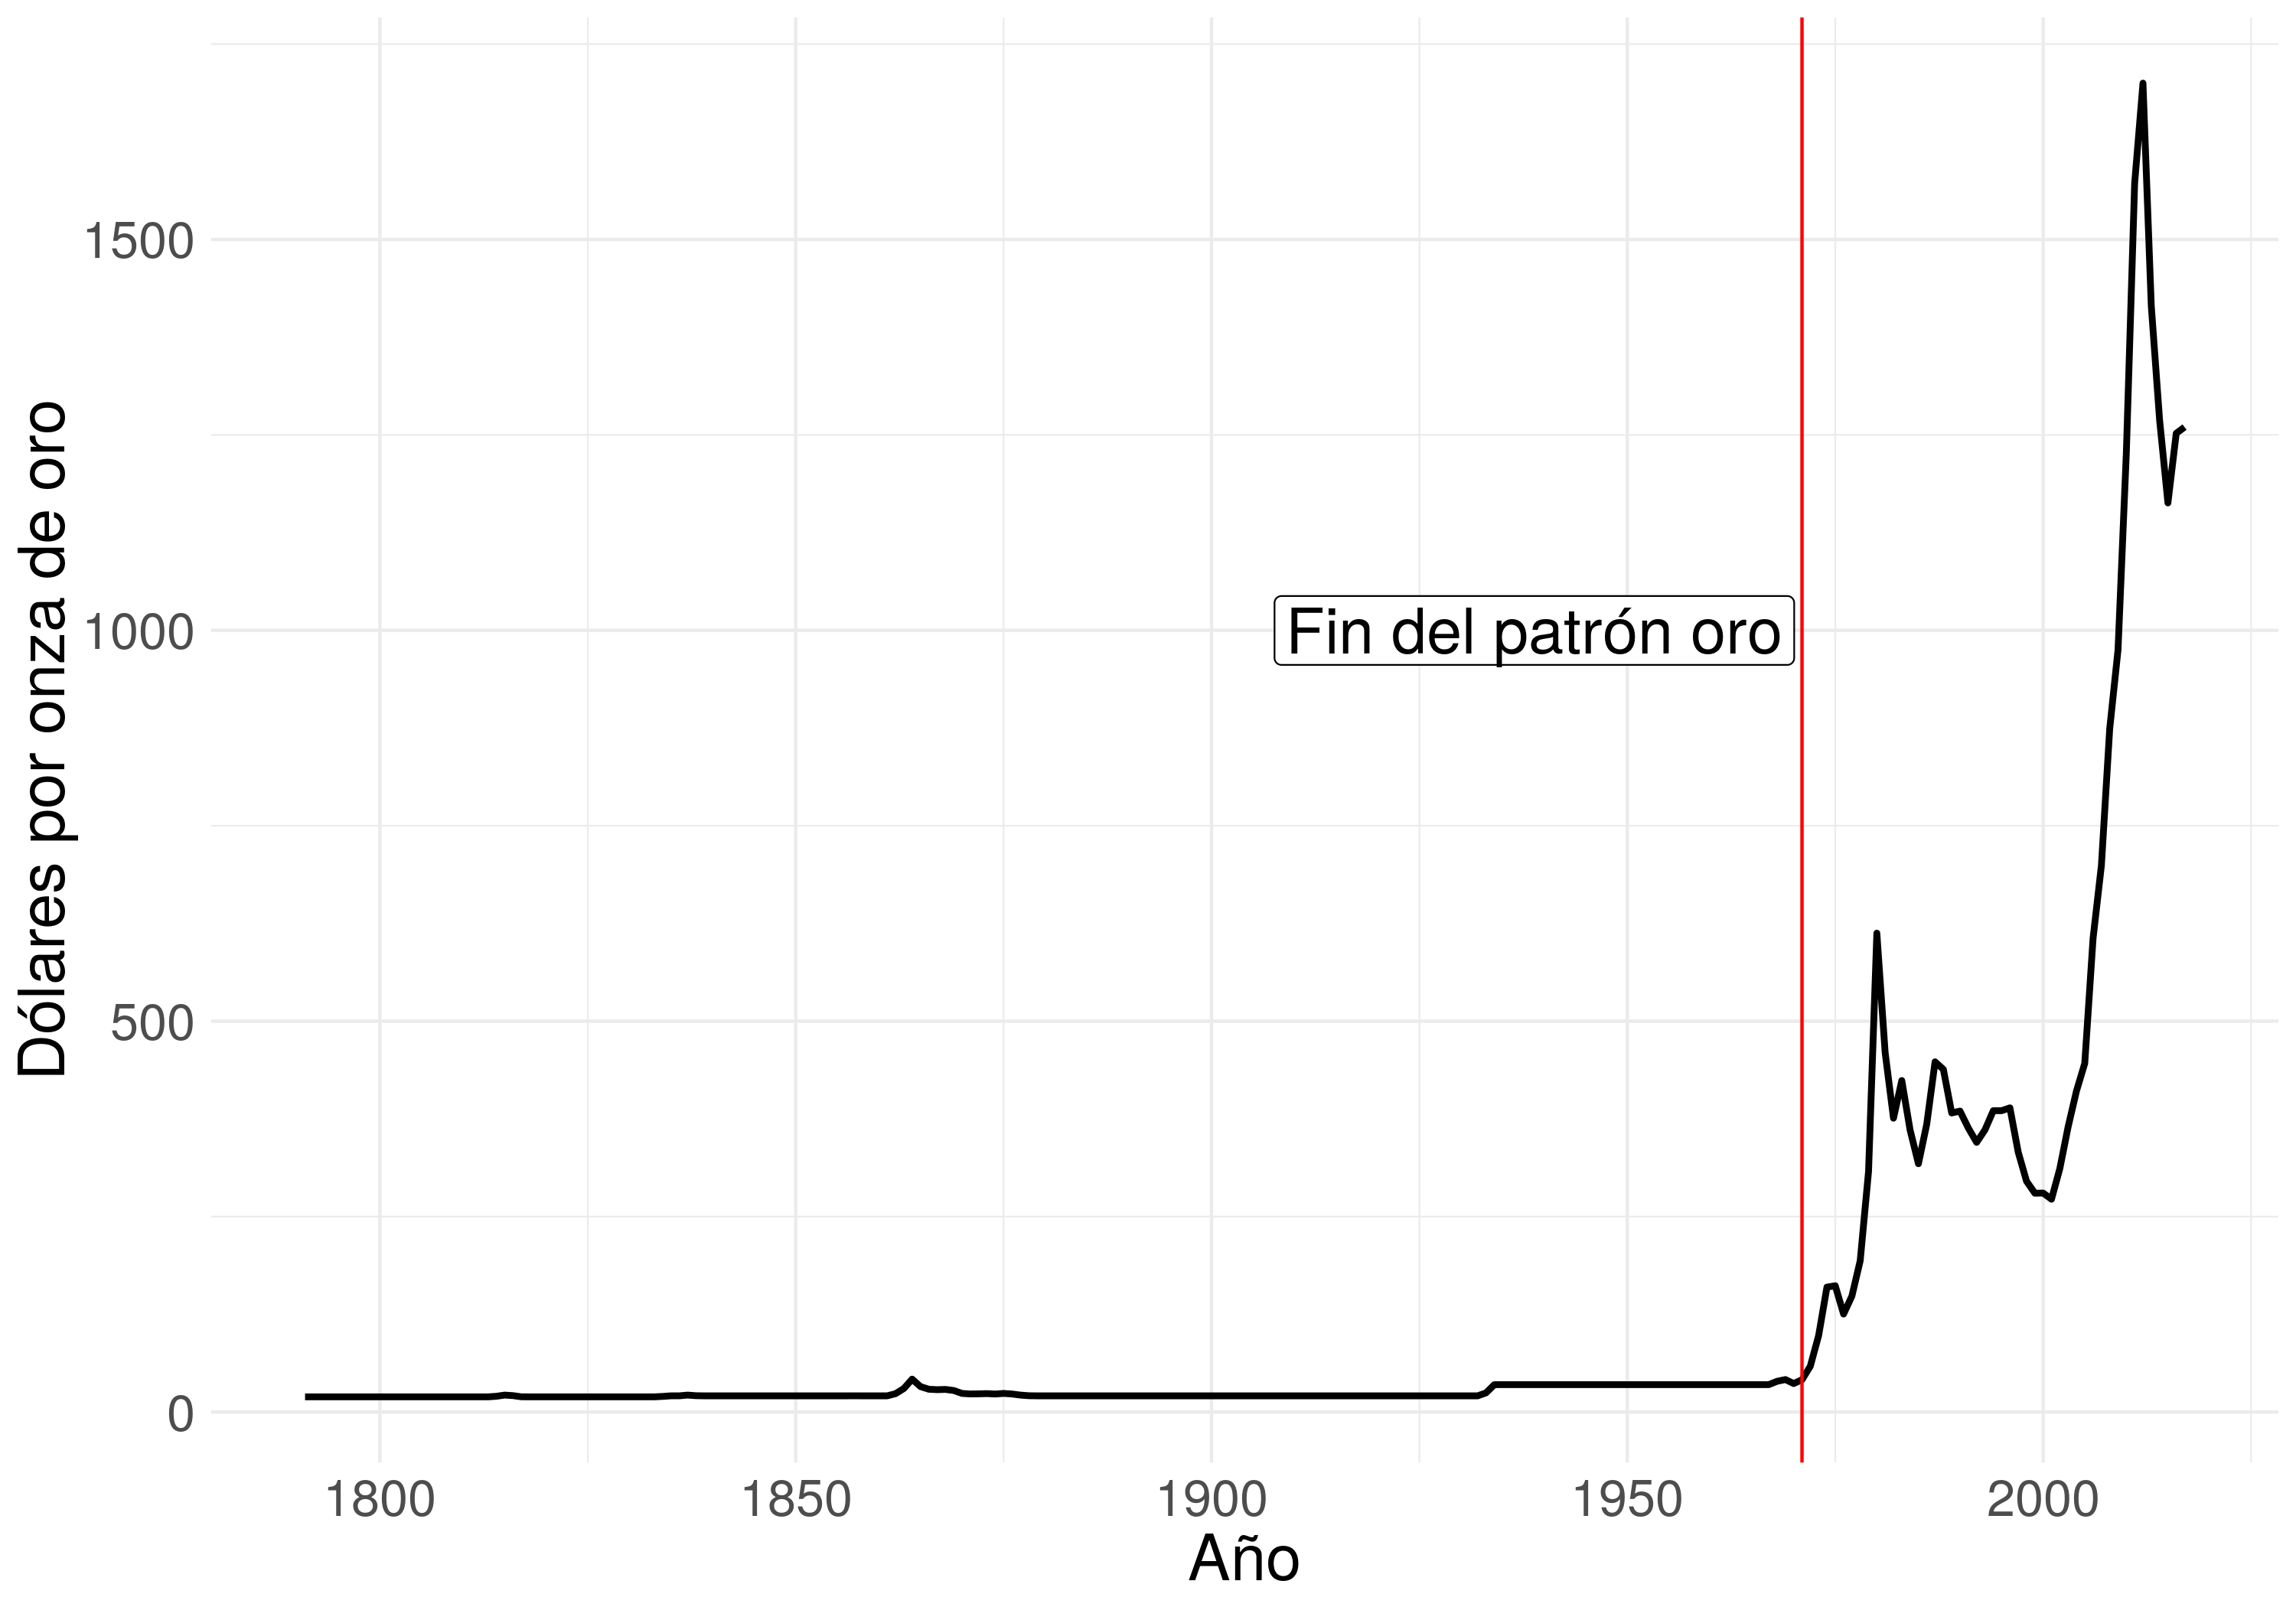
\includegraphics[width=0.8\linewidth]{oro.png}
	\caption{Precios del oro por onza en el mercado de Nueva York} \label{fig:oro}
\end{figure}

Dado que lo que se busca en el presente trabajo es realizar un análisis de largo plazo del ciclo económico, esta perturbación nominal oscurece el fenómeno subyacente que se esta buscando. Es por ello que se opto por normalizar las series del PBI y el salario por el precio del oro. De esta forma las series se leen como el producto y el salario expresado en su capacidad de compra de oro. Una alternativa a esto sería dividir por el Indice de Precios al Consumidor, de forma tal que ambas series se expresen en capacidad de poder adquisitivo constante. Sin embargo, dado que el precio de las mercancías no esta determinado exclusivamente por fenómenos de tipo nominal, tal como la relación dólar-oro, sino por los cambios tecnológicos,y estos últimos juegan un rol central en el desenvolvimiento del ciclo económico, consideramos que esta normalización no sería la adecuada. 

De acuerdo con lo anterior, la figura \ref{fig:PBI} muestra la serie de el PBI de Estados Unidos entre el 1900 y 2017, expresado en oro. Por su parte la figura \ref{fig:salario} muestra la serie del salario horario de un obrero de la producción en Estados Unidos entre 1900 y 2017, expresado en Oro. En ambos casos se resaltan en rojo los períodos de crisis conocidos en la literatura económica, y en líneas punteadas aquellas crisis puntuales que se extienden en un año en particular.

\begin{figure}[H]
	\centering
	\subfigure[PBI expresado en Oro]{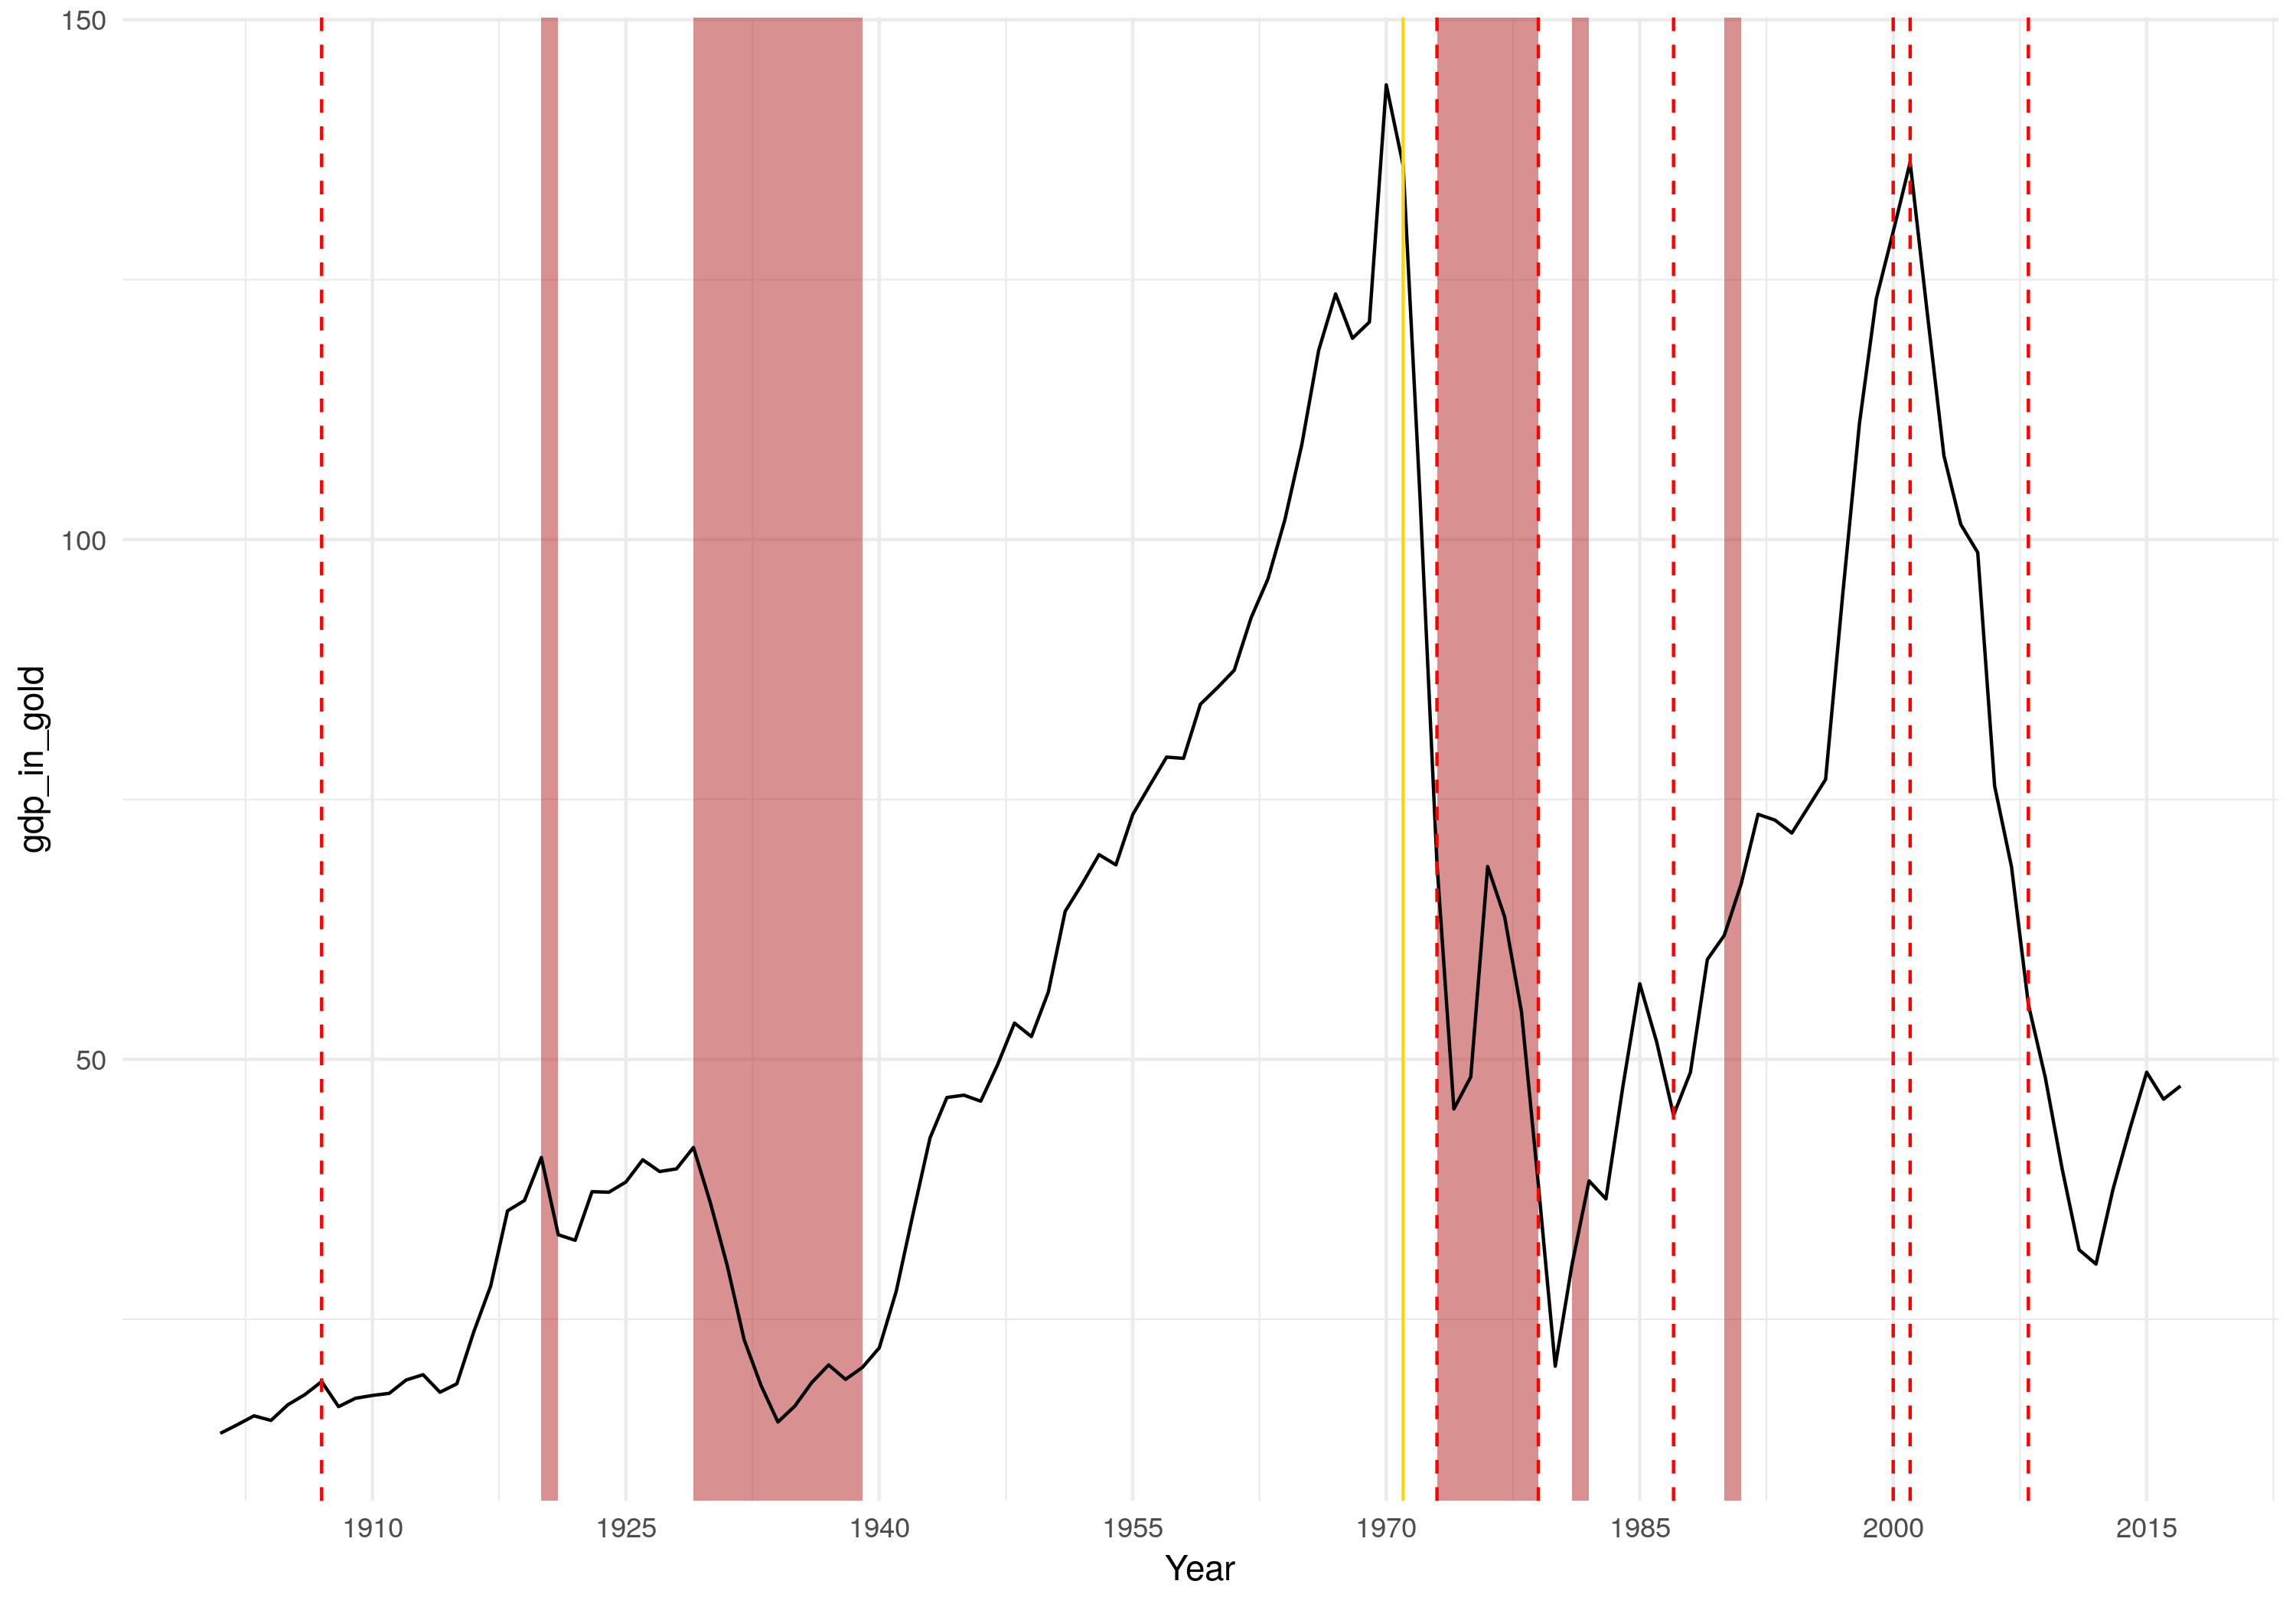
\includegraphics[width=0.75\linewidth]{gdp_in_gold_eda.PNG}
	\label{fig:PBI}}
	\subfigure[Salario expresado en Oro]{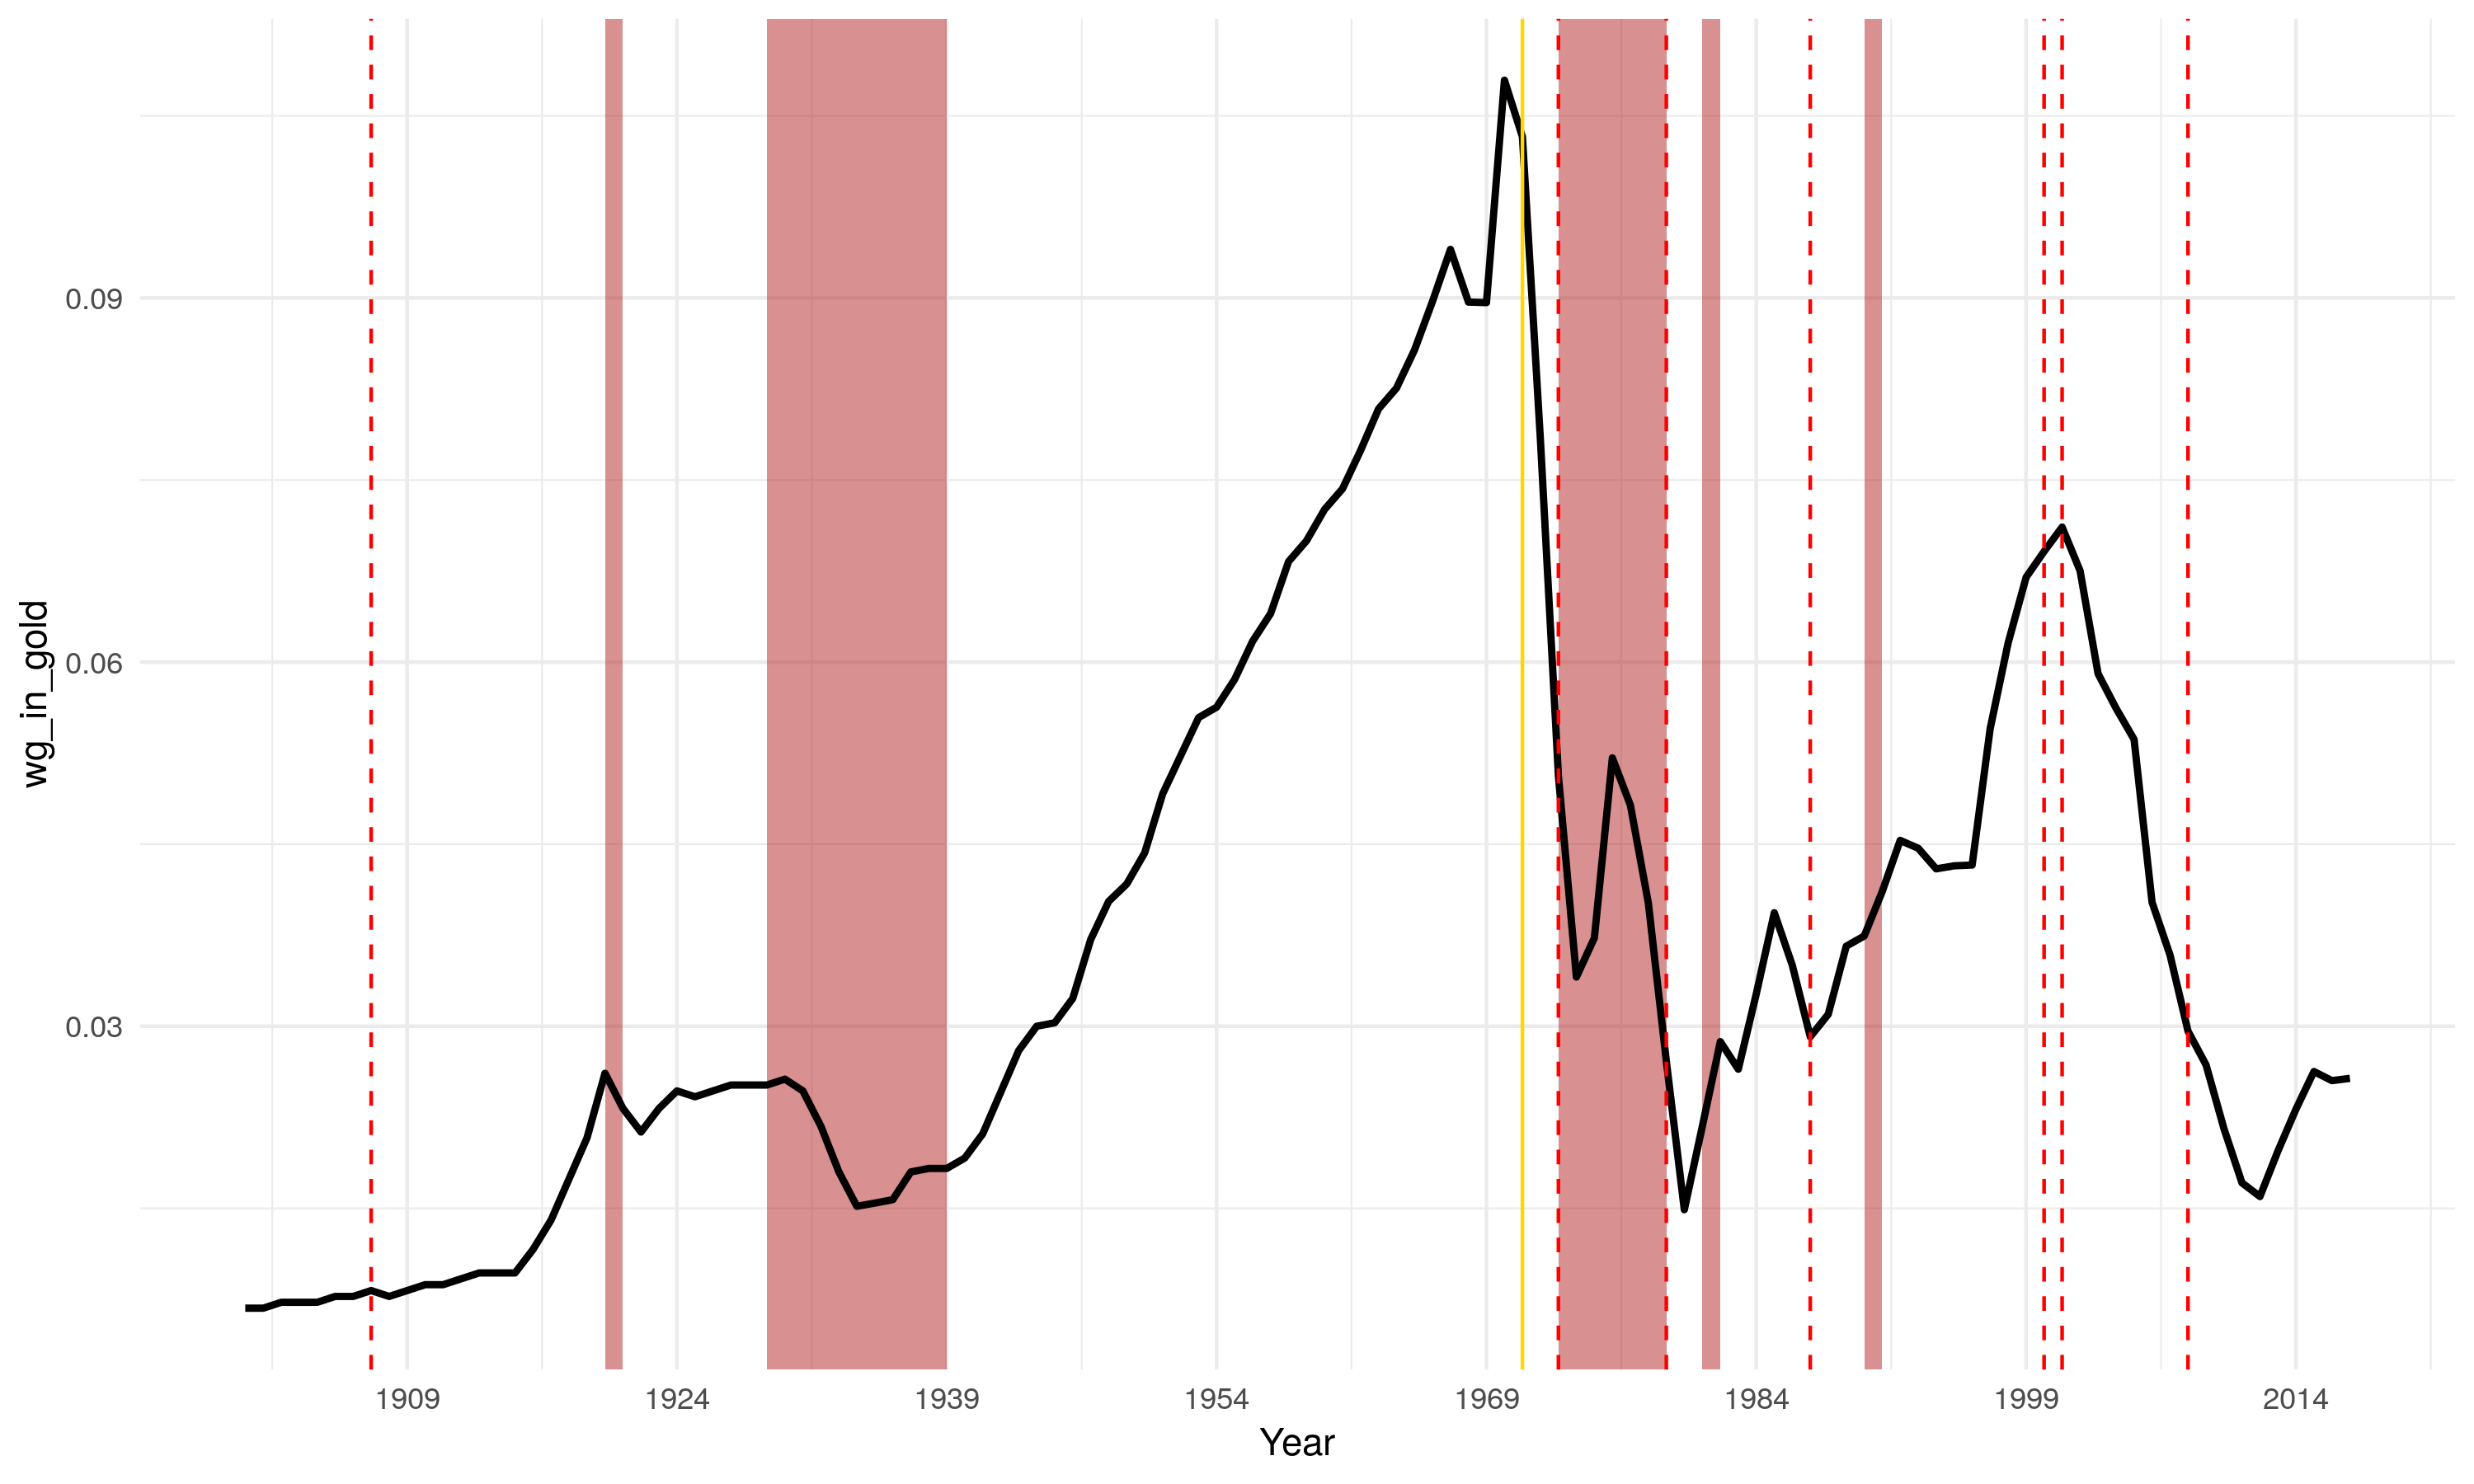
\includegraphics[width=0.75\linewidth]{wg_in_gold_eda.PNG}
	\label{fig:salario}}
	\caption{Series Expresadas en Oro. Destacado de crisis conocidas} \label{fig:series_crisis}
\end{figure}

En primer lugar lo que se observa es la similitud de ambas series, en términos generales. Ambas muestran tres picos, durante los 20', en 1970 y el 200, seguidos de caídas profundas. La normalización por el precio del oro permite ver un gran ciclo con tres oscilaciones, por lo menos de manera aparente, durante el siglo XX. Las crisis revisadas por la literatura de historia económica parecen tener su correlato en los movimientos observados en ambas series. Por su parte, también es interesante resaltar que el tercer movimiento ascendente, cuyo punto álgido se encuentra en el año 2000, lleva a un valor similar al del movimiento oscilatorio previo para el caso del PBI, pero no para el salario. Esto expresa que la distribución del PBI en salario y ganancia se modificó en el último período. 


\section{Autocorrelación y ARIMA}

En la presente sección se analizará la autocorrelación de las series anteriores, para observar su comportamientos desde un punto de vista sistemático. Para ello también se observará un modelo ARIMA. 

En primer lugar, se calculó la autocorrelación para el total del período en ambas series. Esto se puede observar en la figura \ref{fig:autocorrelacion_tot}. Ambas series tienen un comportamiento similar, con una fuerte correlación con el período anterior, una correlación positiva con respecto a 6 lags, y una relación negativa con 10 lags. 

\begin{figure}[H]
	\centering
	\subfigure[PBI expresado en Oro]{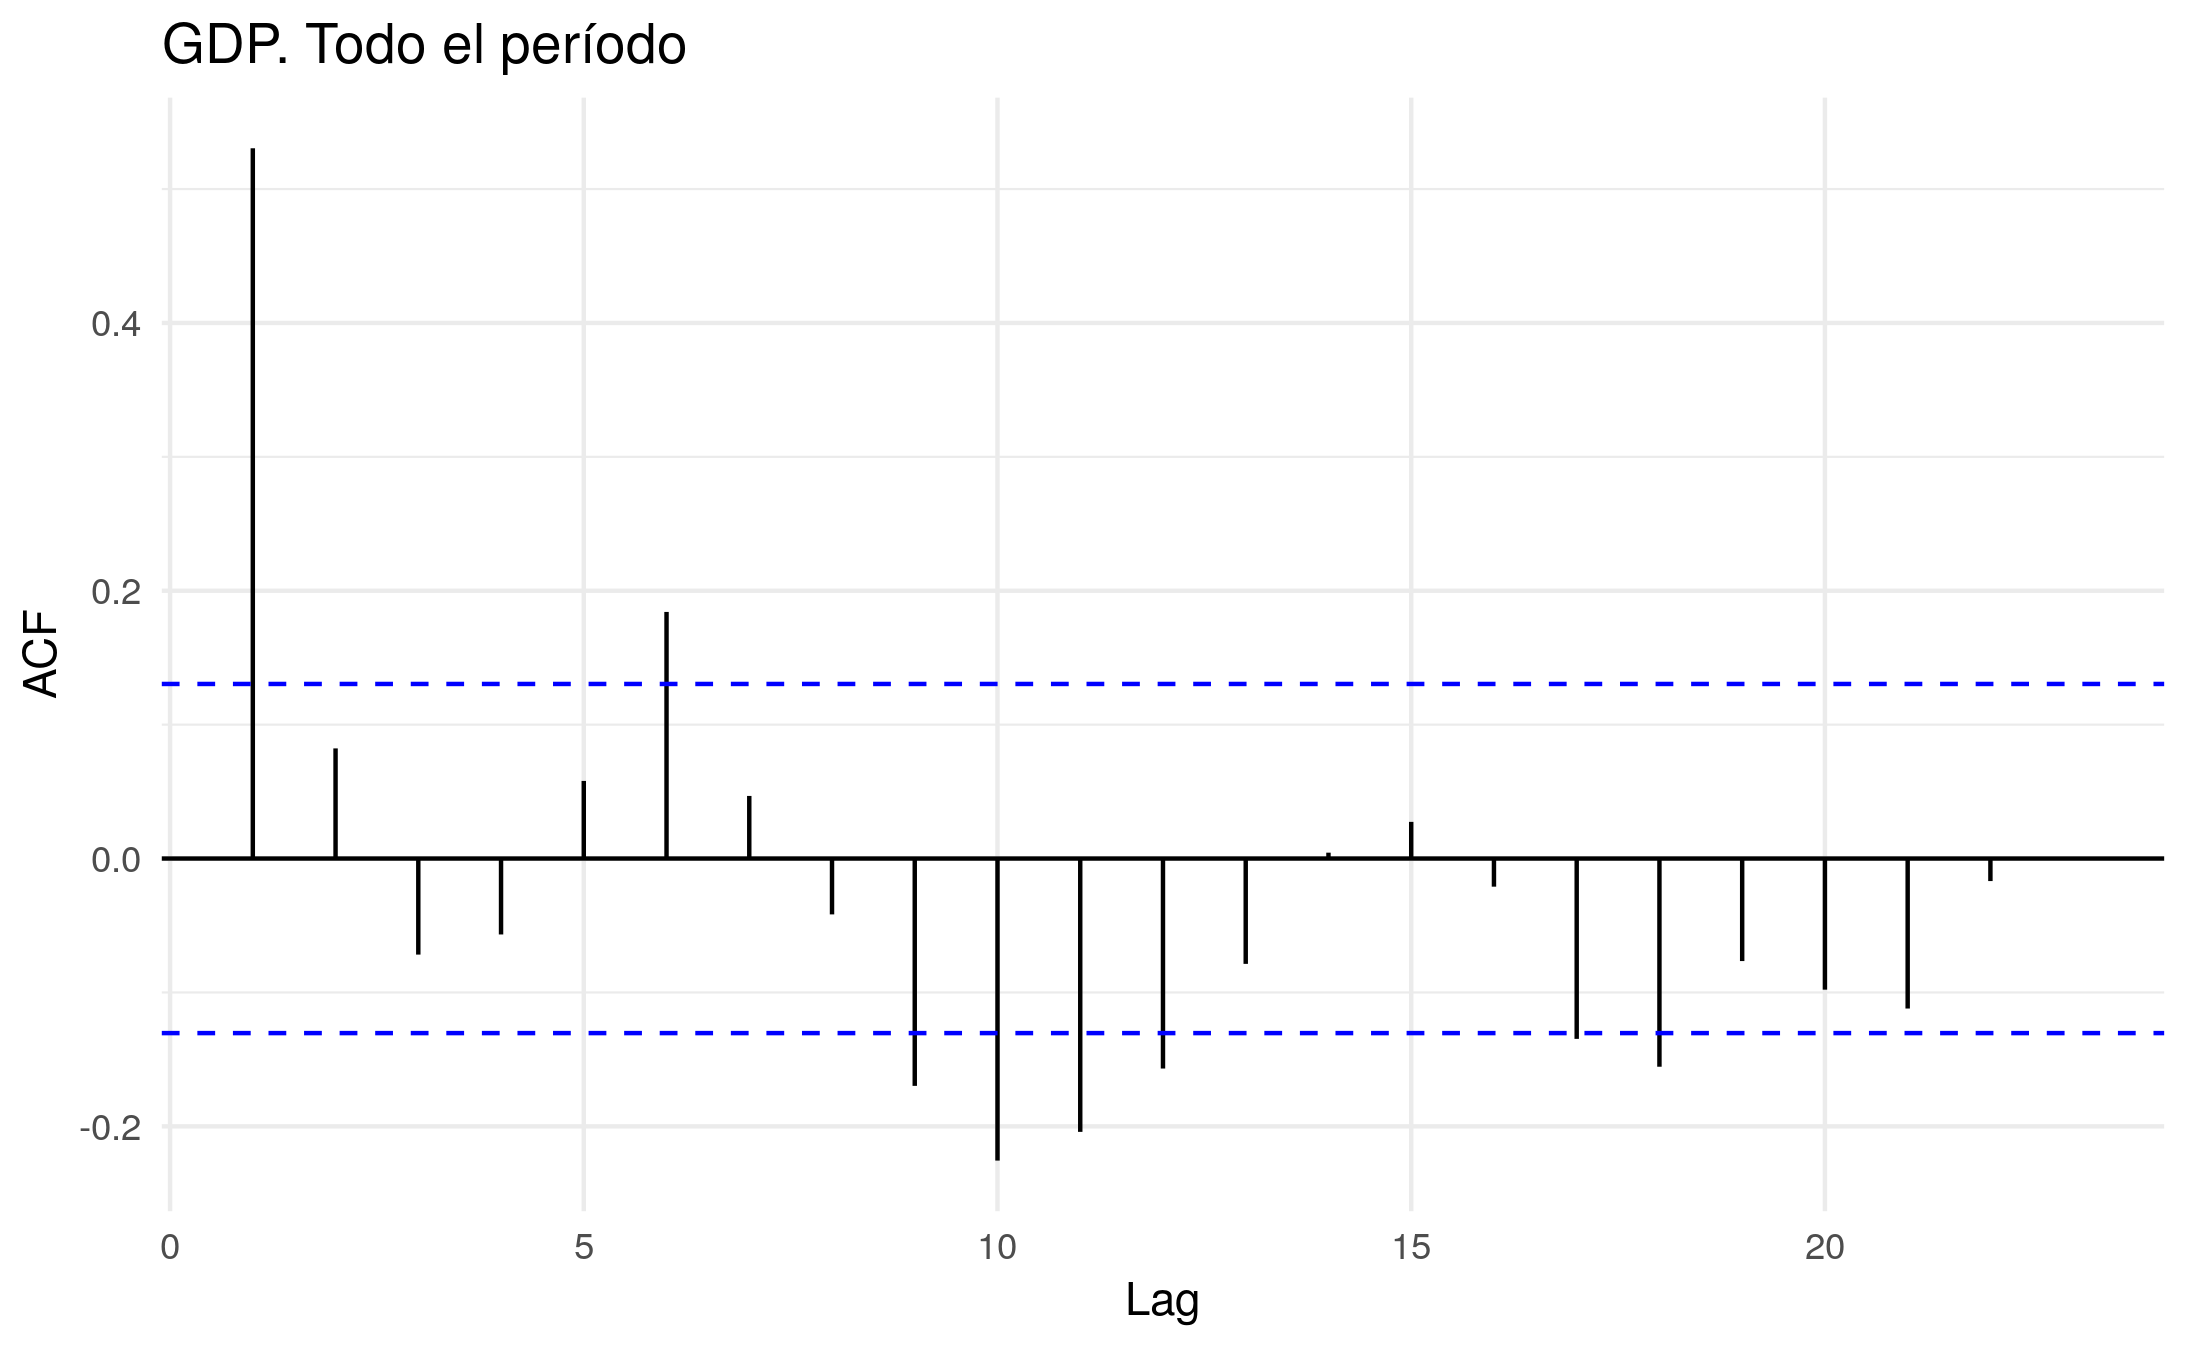
\includegraphics[width=0.75\linewidth]{Autocorrelacion_gdp.png}}
	\subfigure[Salario expresado en Oro]{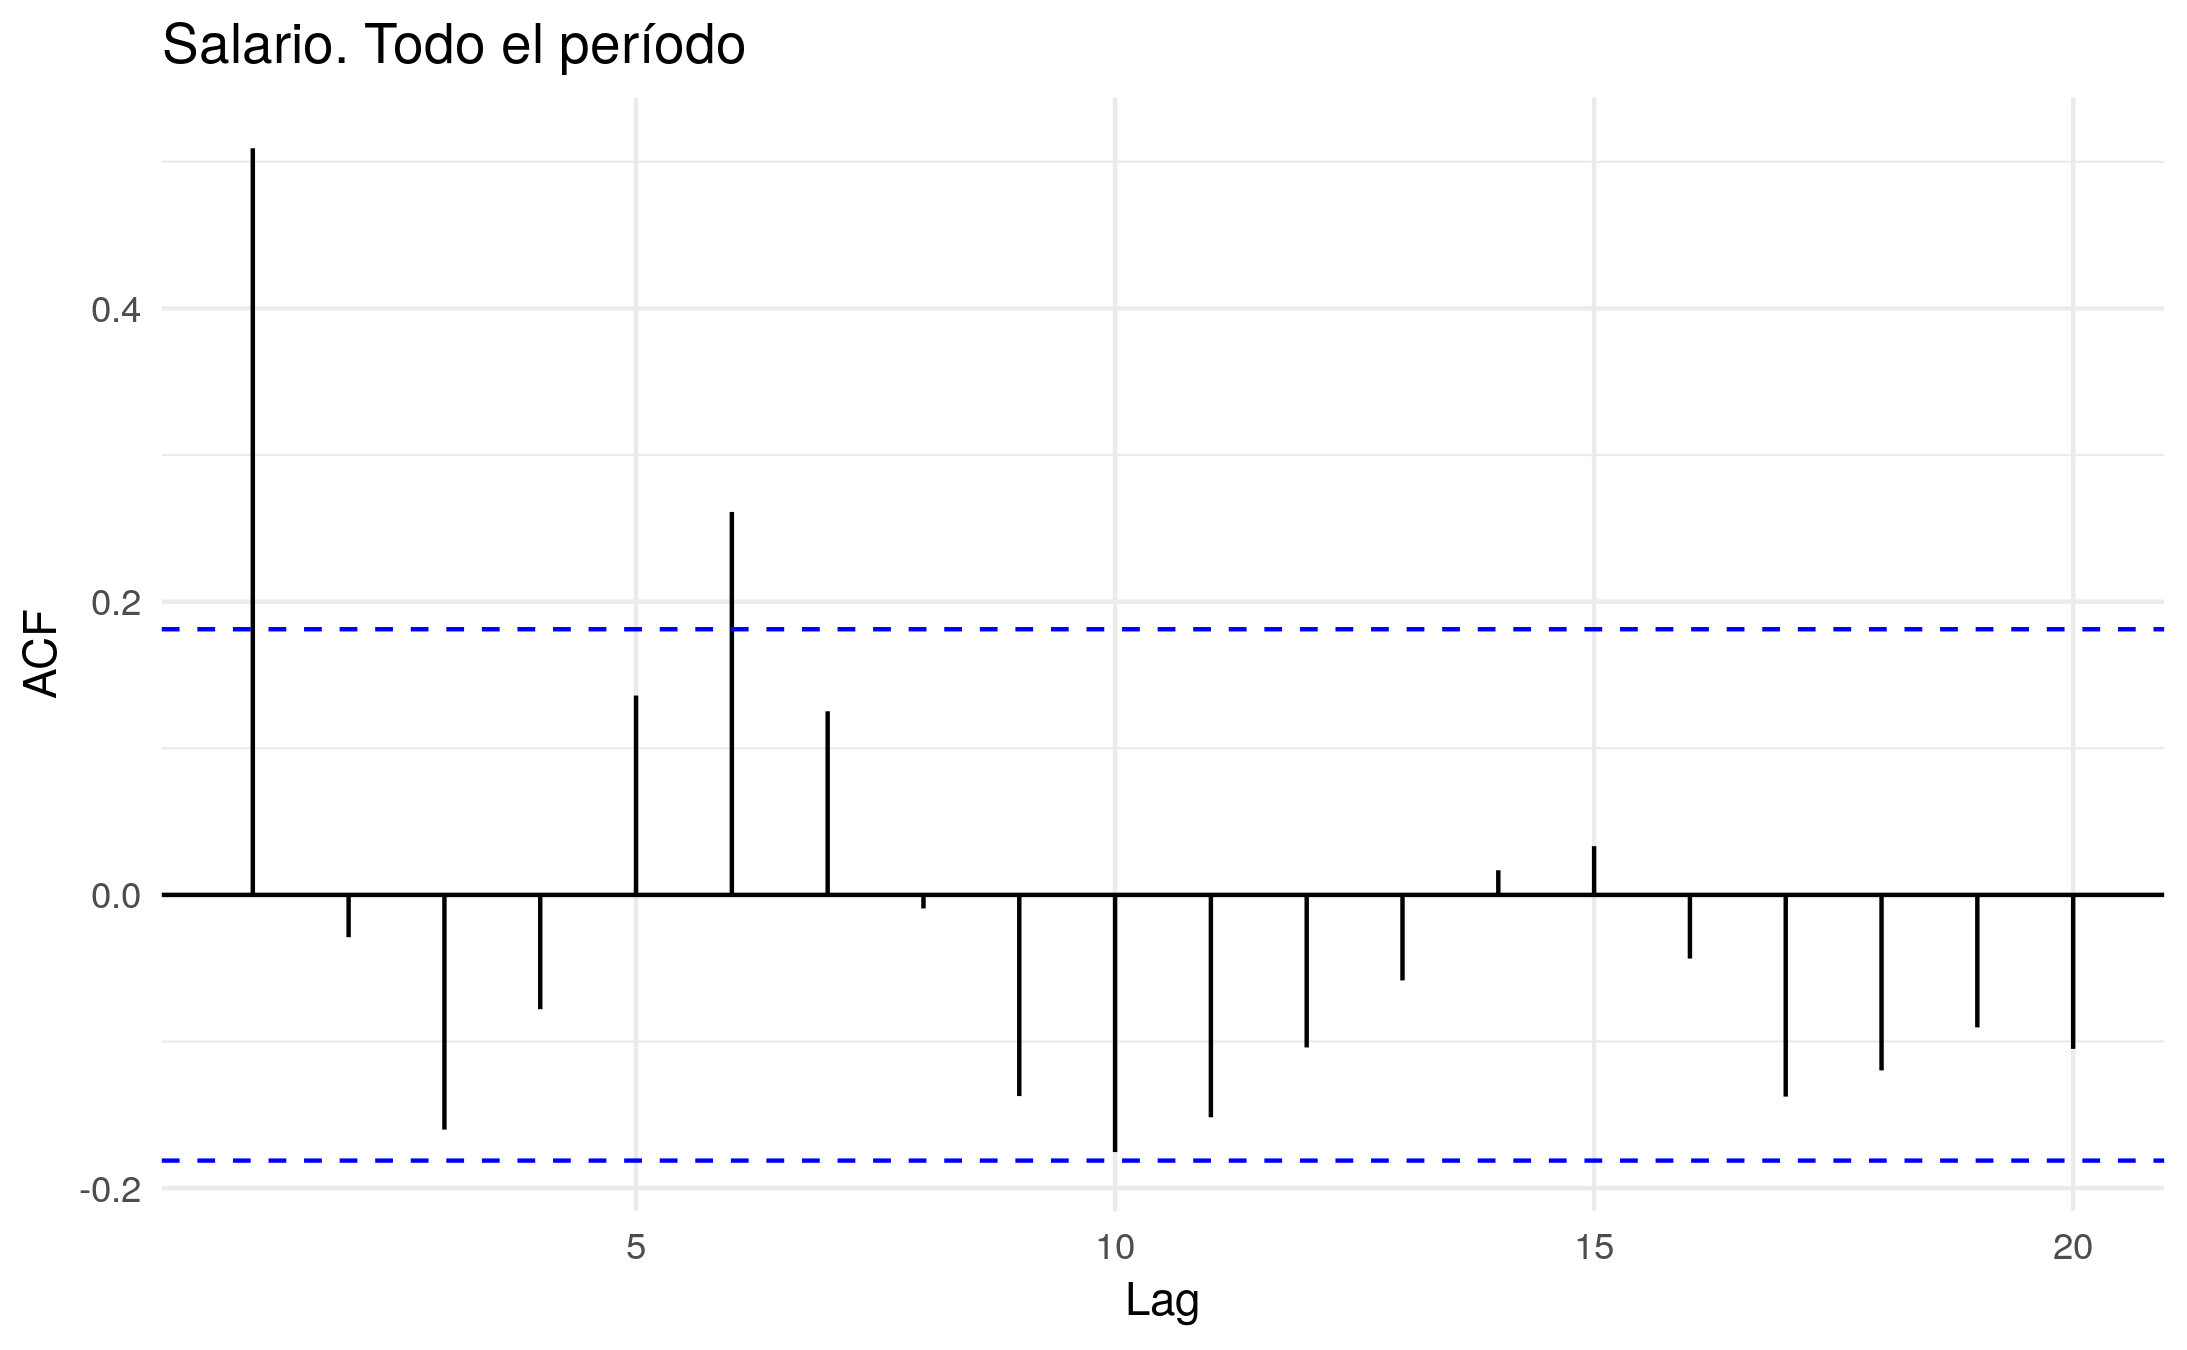
\includegraphics[width=0.75\linewidth]{Autocorrelacion_wg.png}}
	\caption{Autocorrelación de las series} \label{fig:autocorrelacion_tot}
\end{figure}

Si embargo, dada la importancia de la caída del patrón oro en el 71', se decidió recalcular las autocorrelaciones para antes y después de dicho año. Esto puede observarse en la figura \ref{fig:autocorrelacion_grp}. Aquí nuevamente las series presentan un comportamiento similar entre sí, y sin embargo muy distinto antes y después del período. En particular, antes de 1971 se observa una fuerte correlación positiva con períodos anteriores, en particular para el PBI, que mantiene una relación positiva con hasta los 12 primeros lags. Esto esta reflejando una fuerte tendencia ascendente. Es importante considerar que el quiebre de la serie se realiza en un pico, por lo que antes del 71' queda un fuerte crecimiento observado desde la segunda guerra mundial hasta dicho punto. Lo notable es que ambas series luego de este punto sólo muestran una correlación significativa con el período anterior, es decir parecieran ser un \textit{random walk}.


\begin{figure}[H]
	\centering
	\subfigure[PBI antes 1971]{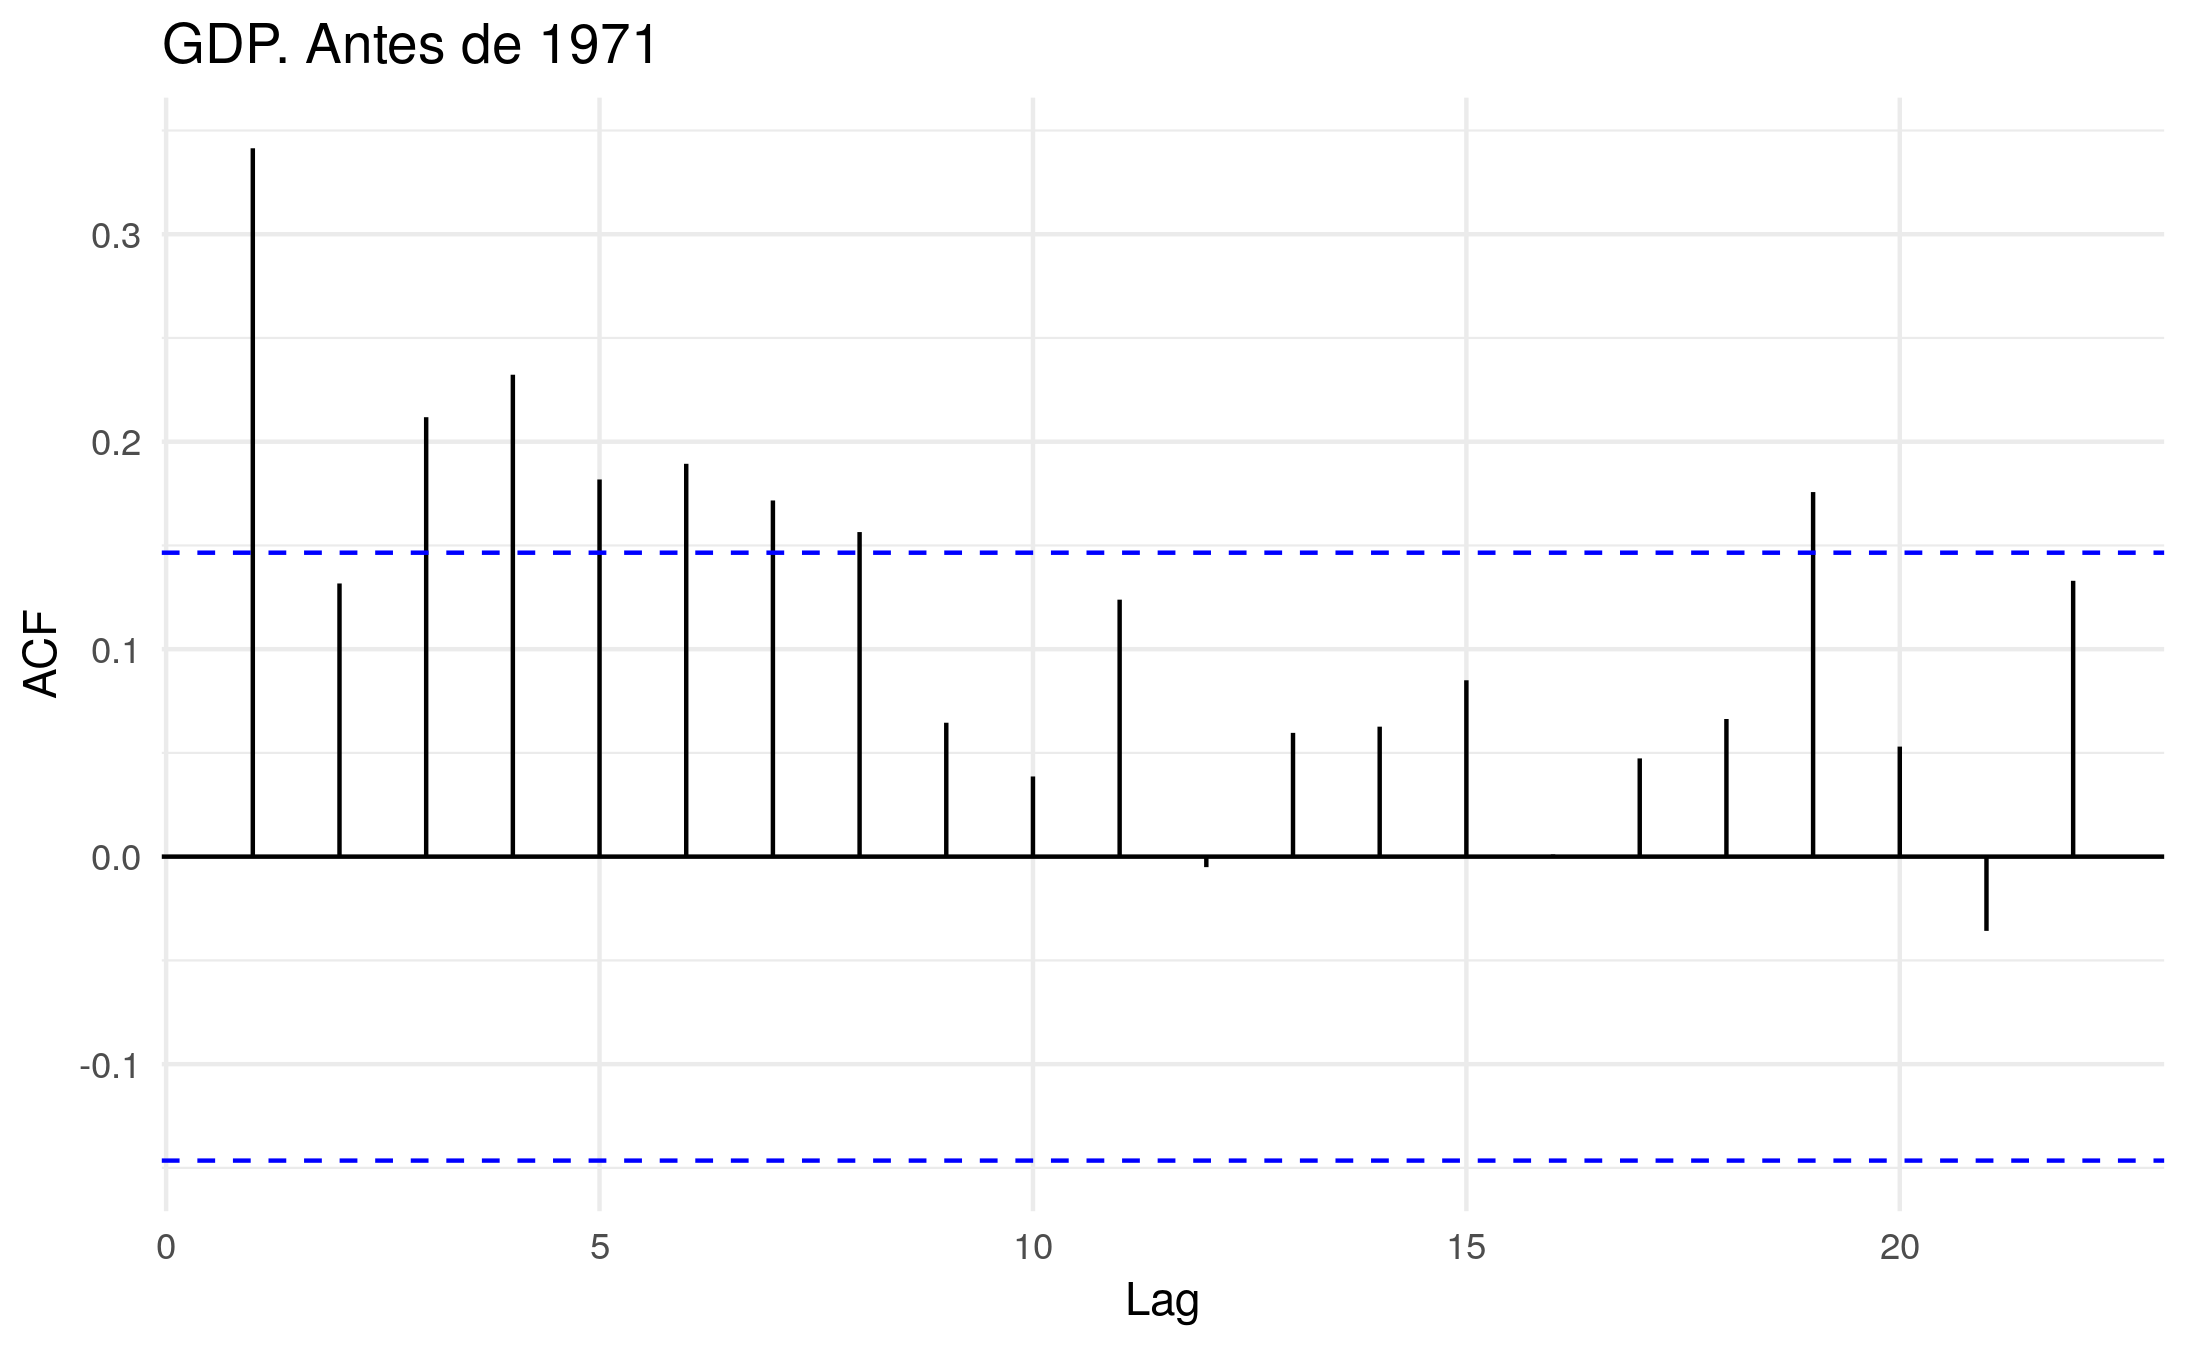
\includegraphics[width=0.49\linewidth]{Autocorrelacion_gdp_pre71.png}}
	\subfigure[PBI después 1971]{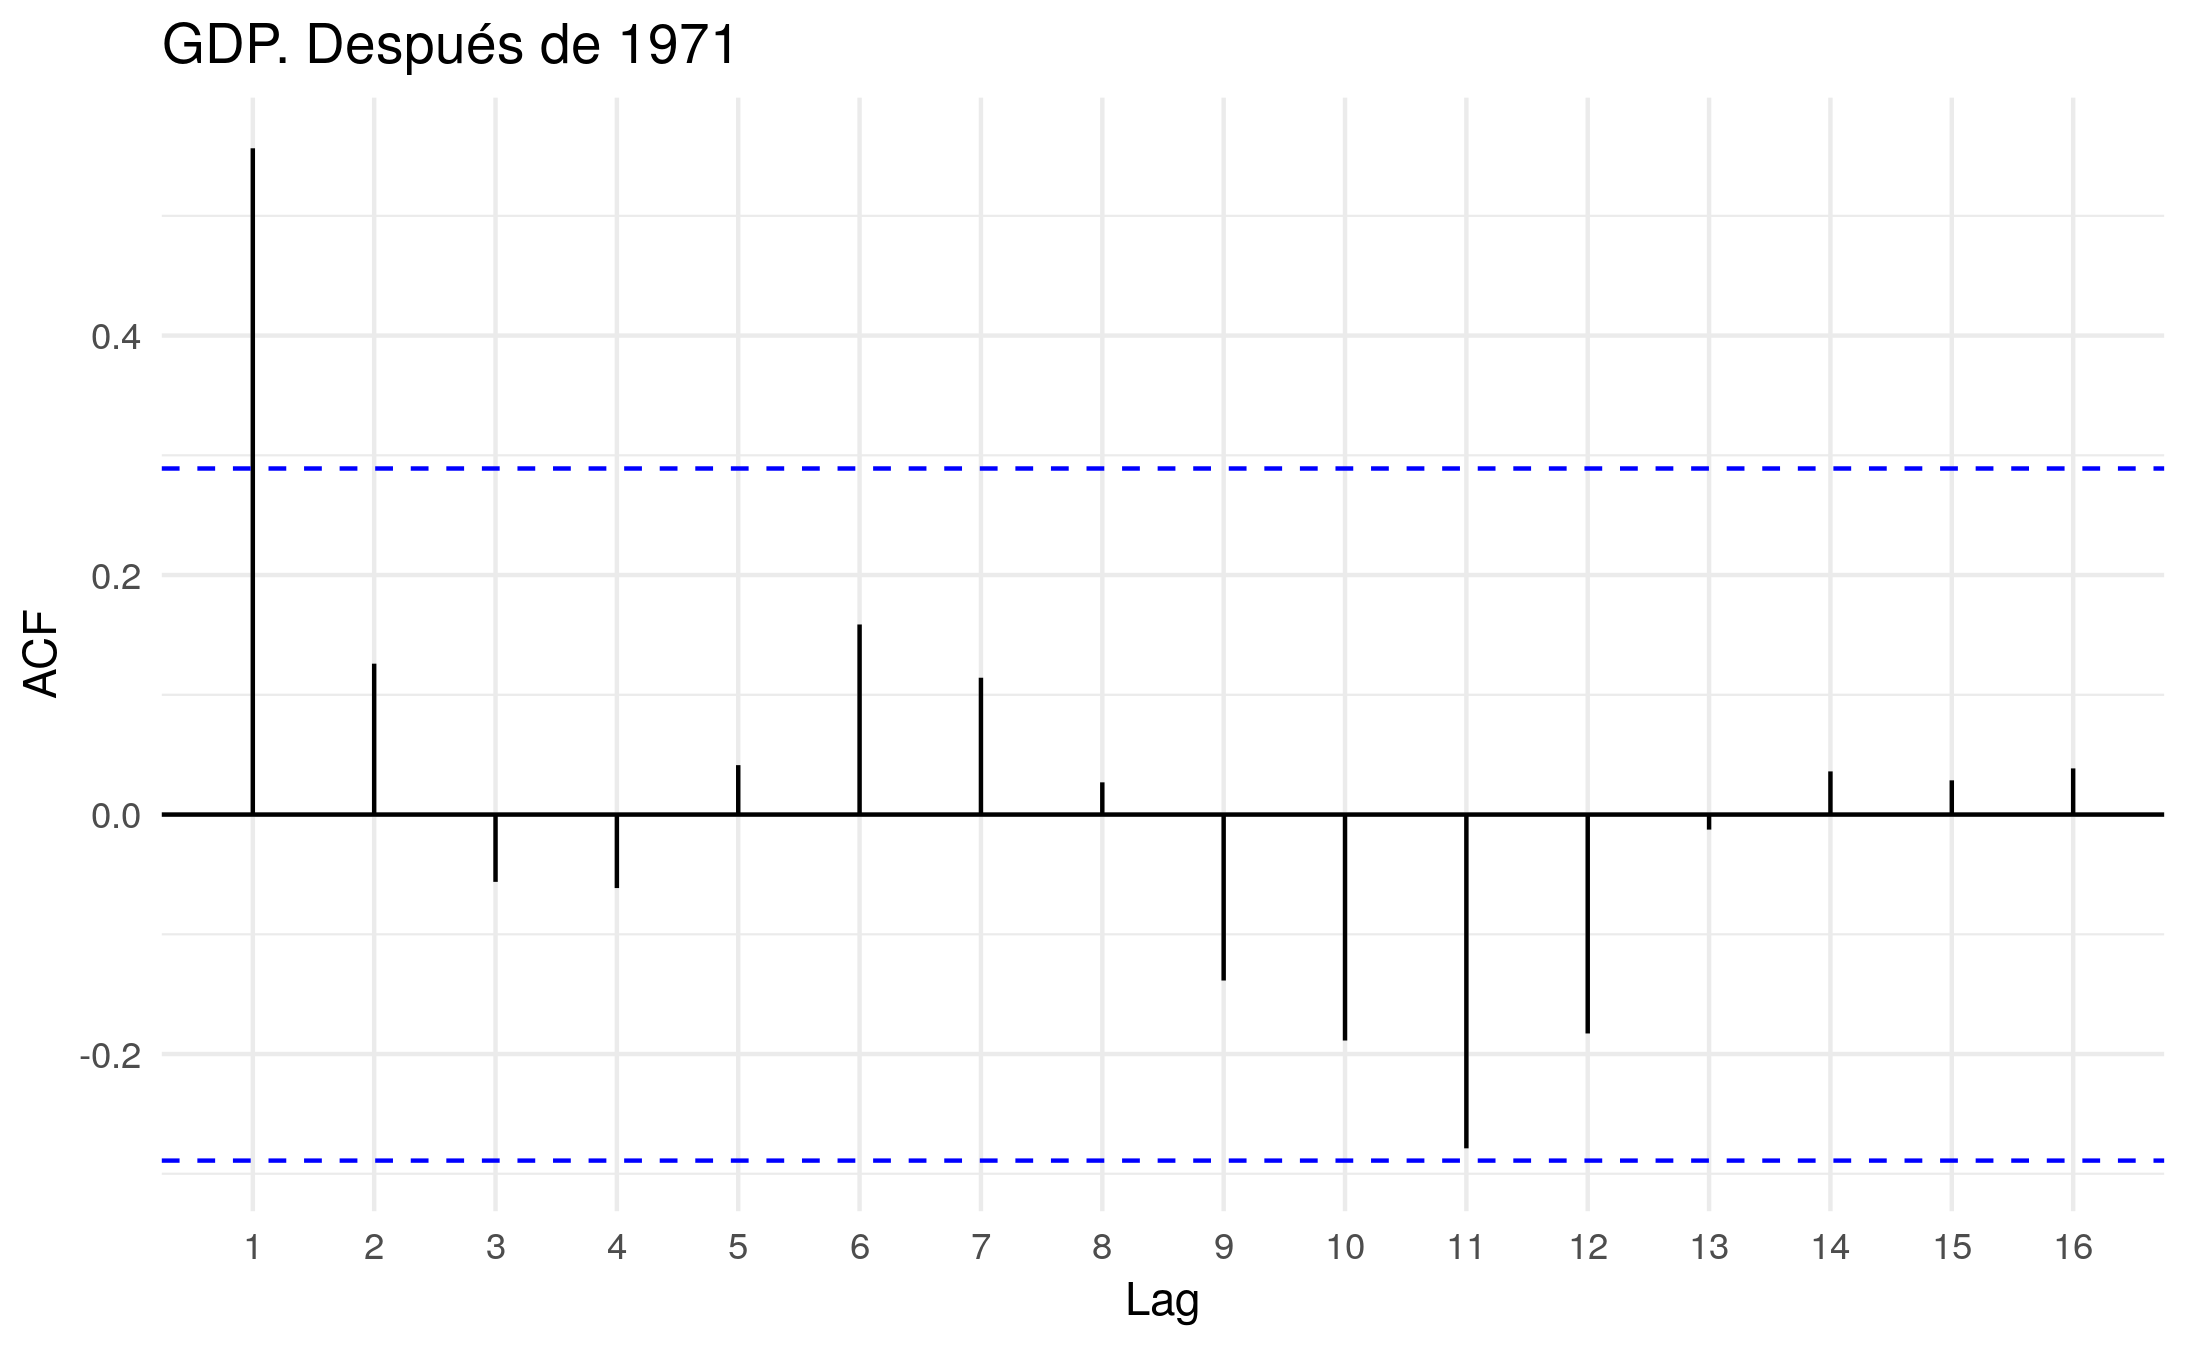
\includegraphics[width=0.49\linewidth]{Autocorrelacion_gdp_post71.png}}
	\subfigure[Salario antes 1971]{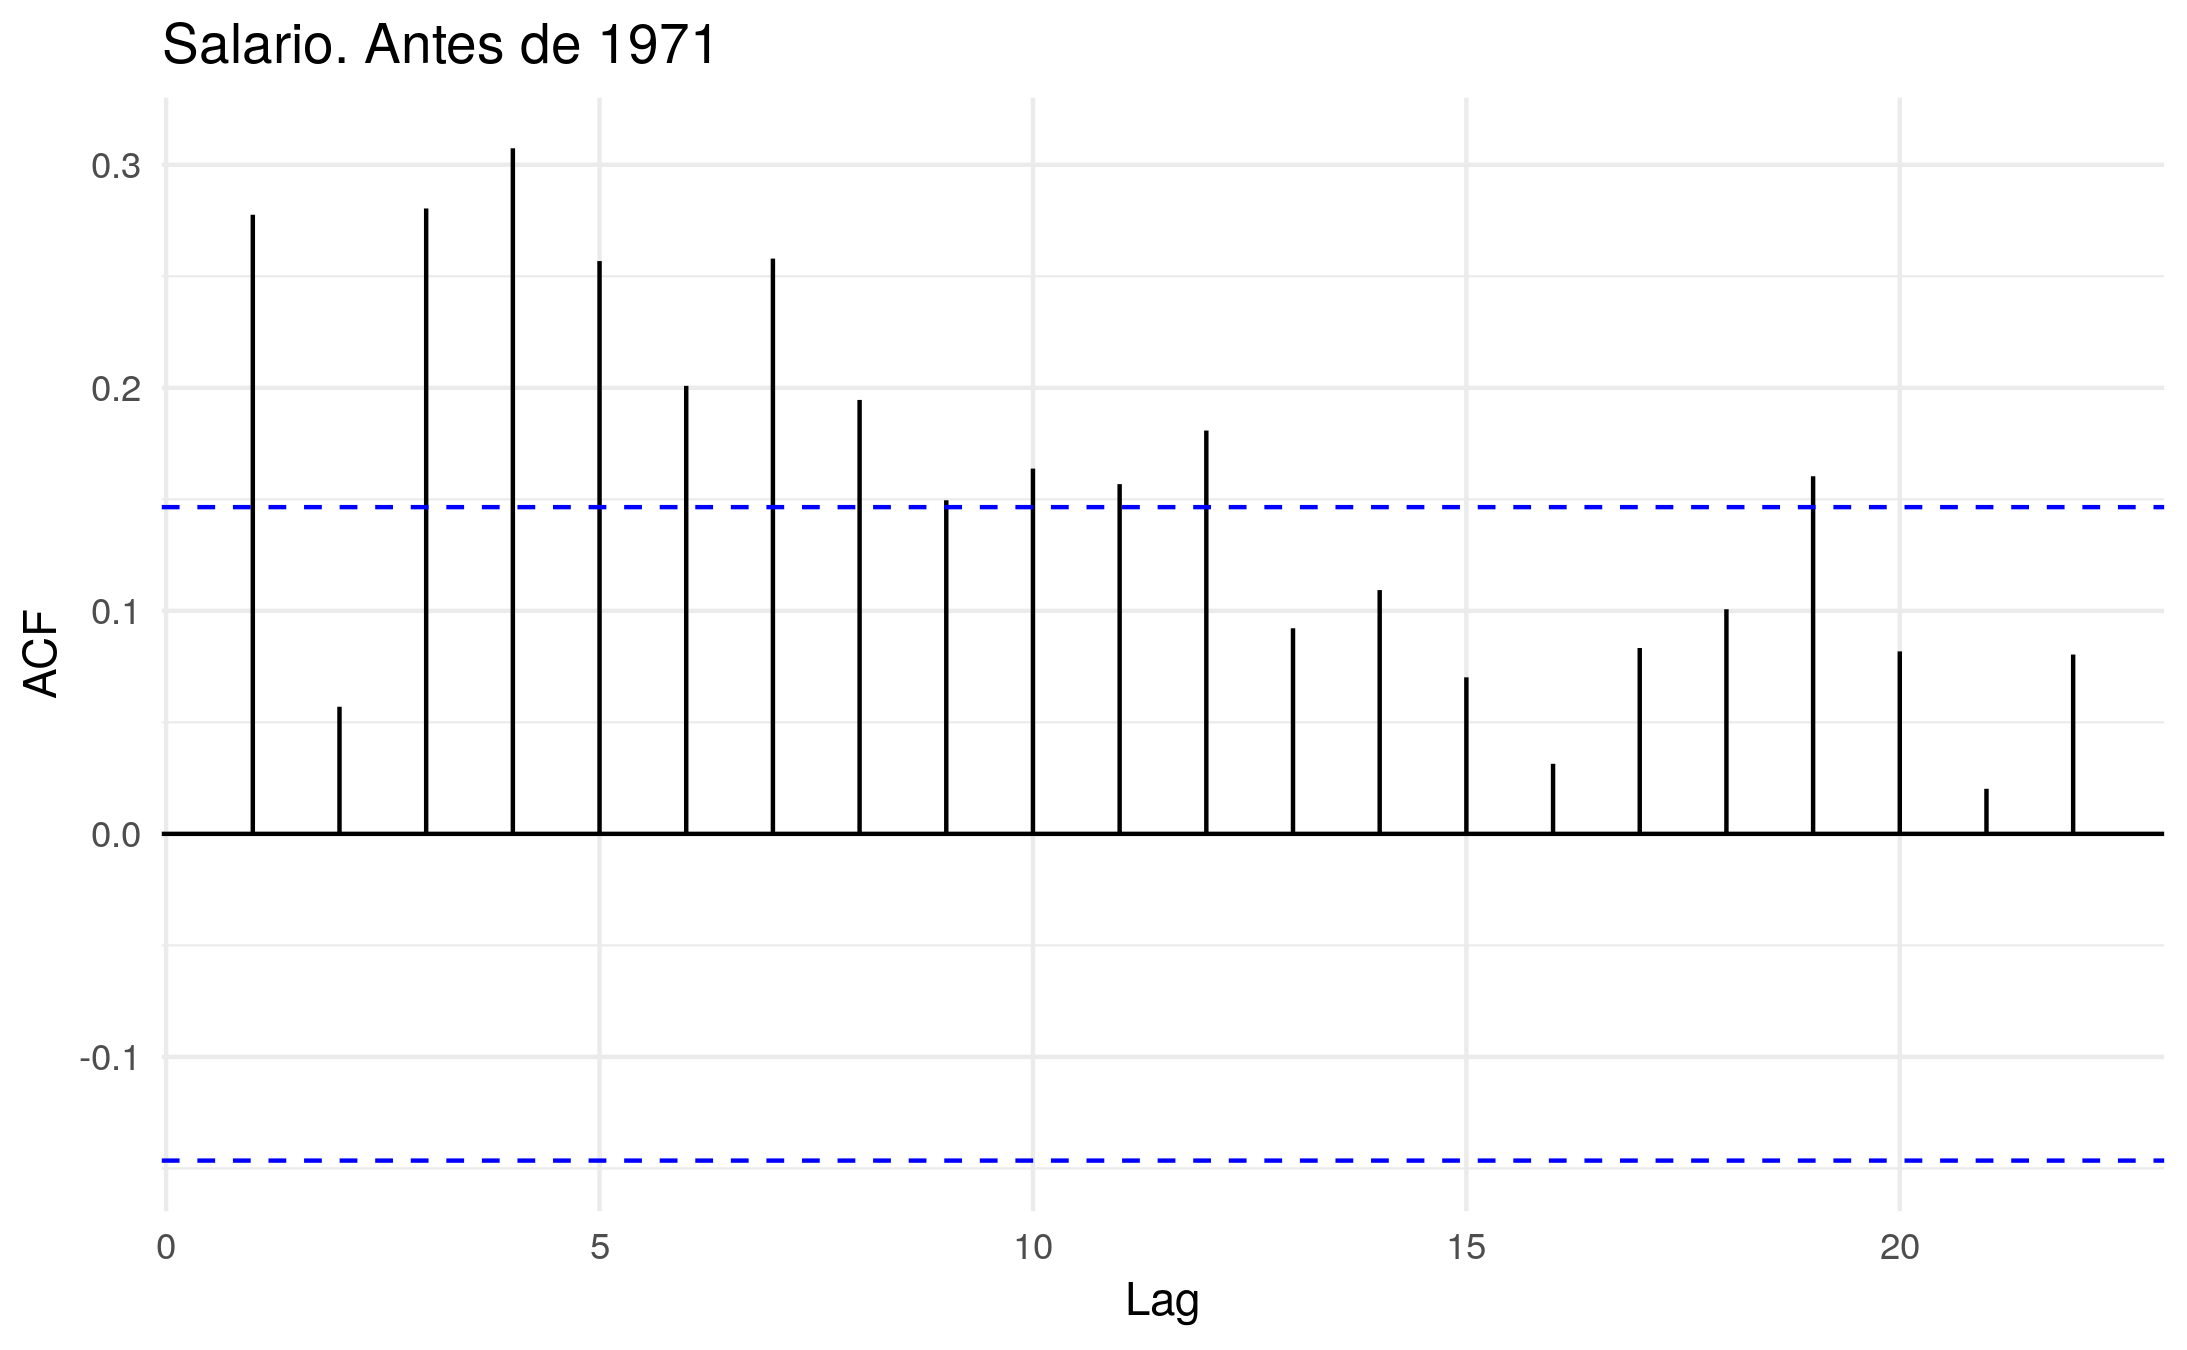
\includegraphics[width=0.49\linewidth]{Autocorrelacion_wg_pre71.png}}
	\subfigure[Salario después 1971]{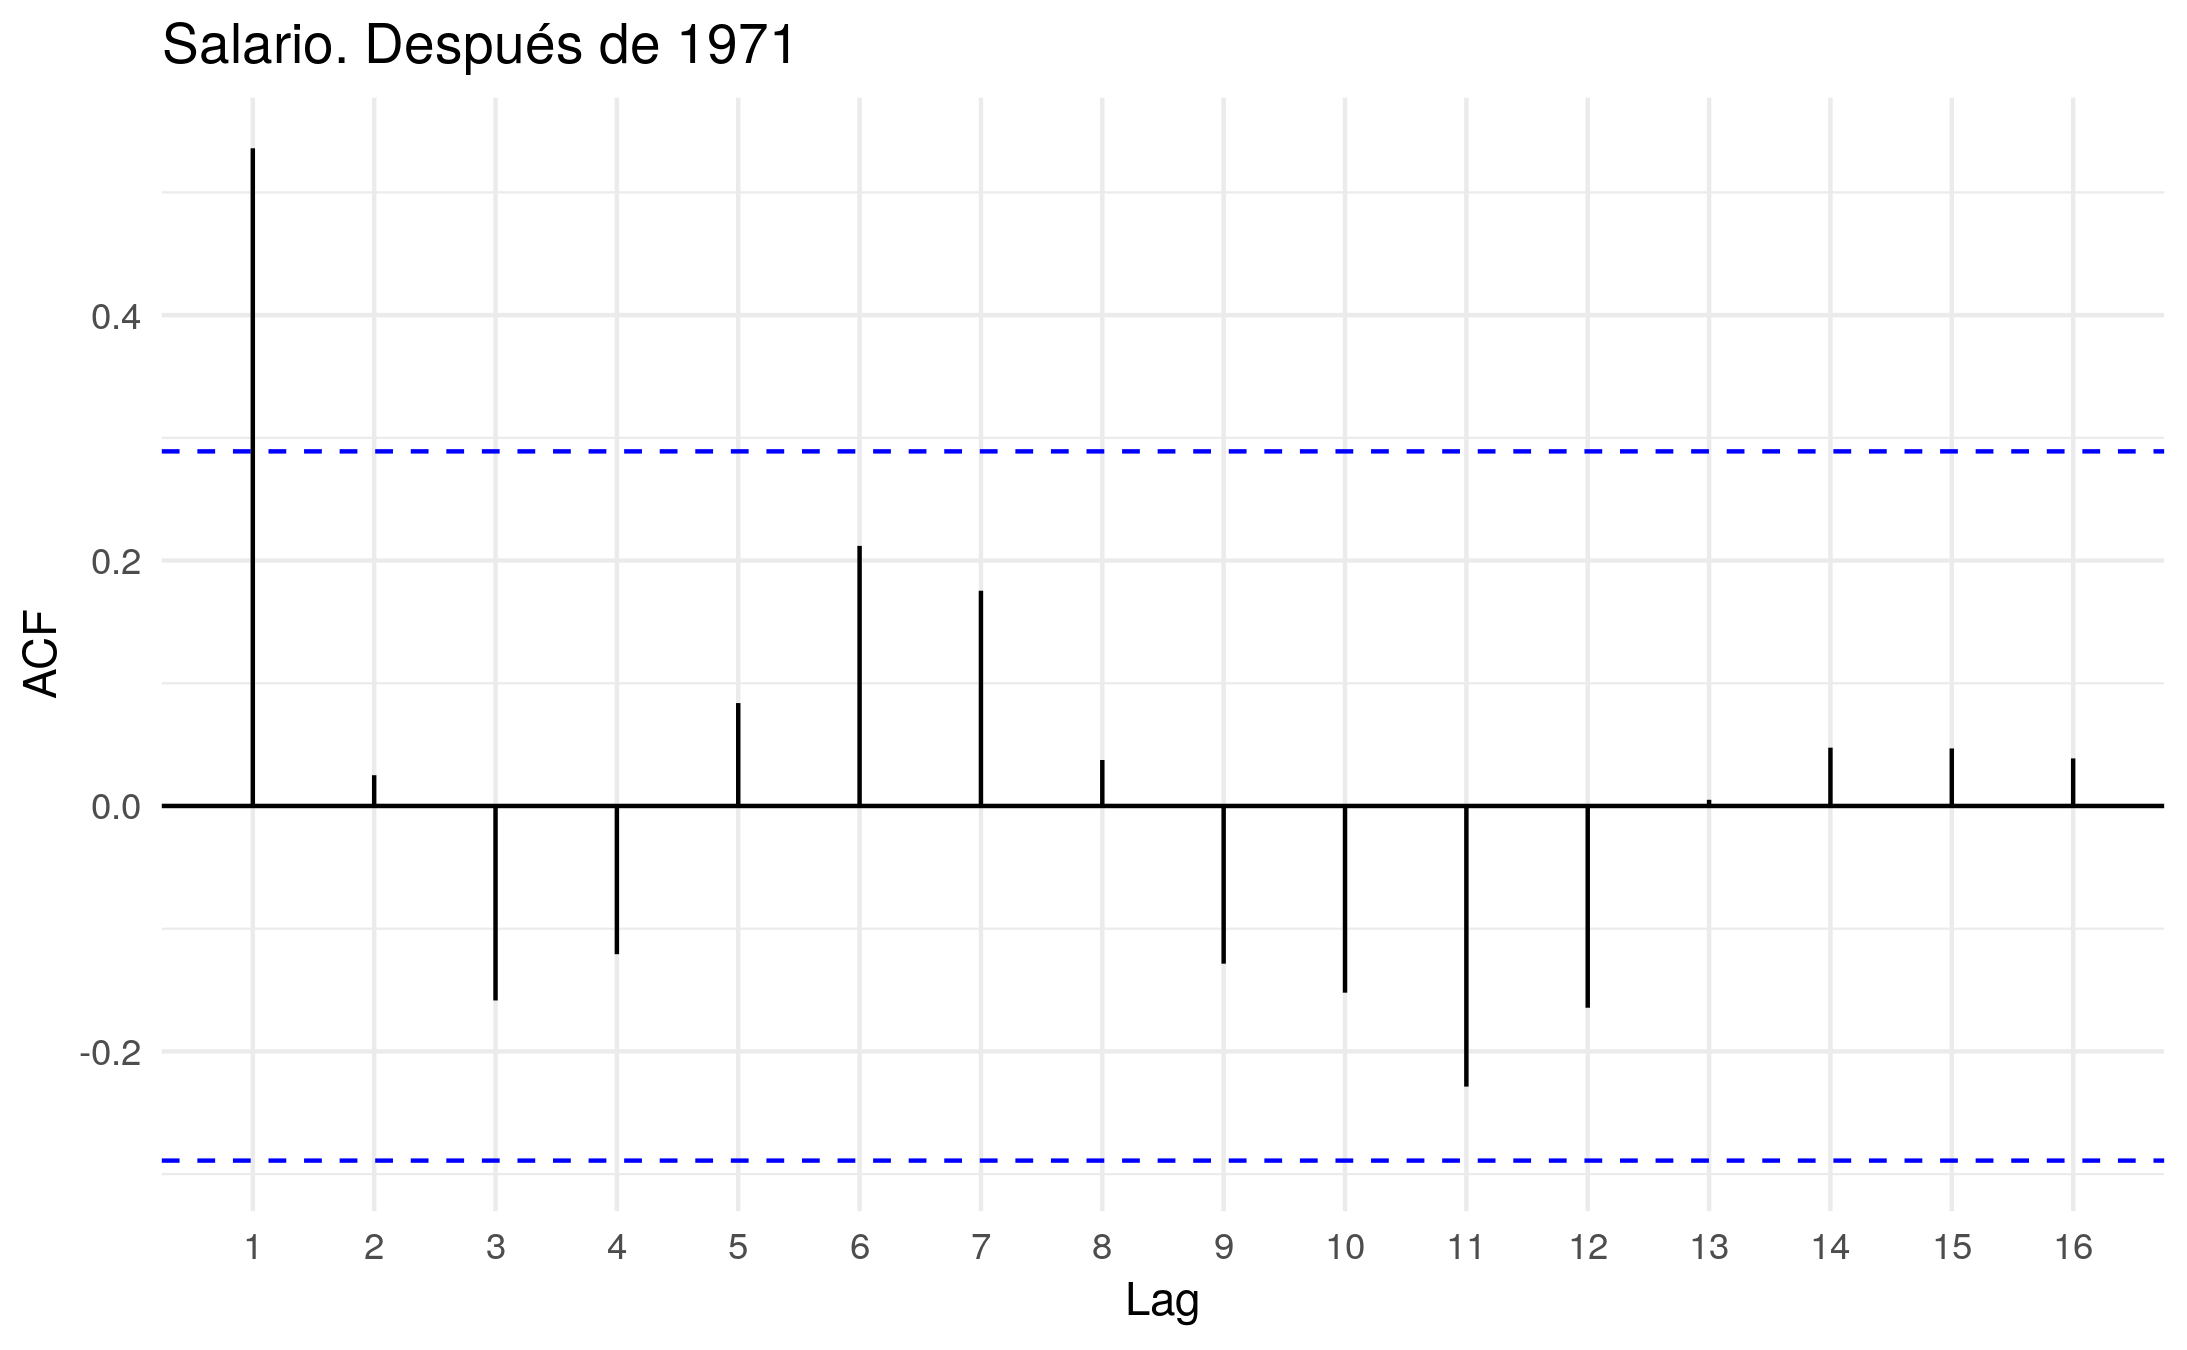
\includegraphics[width=0.49\linewidth]{Autocorrelacion_wg_post71.png}}
	\caption{Autocorrelación de las series} \label{fig:autocorrelacion_grp}
\end{figure}

En la figura \ref{fig:arima} se observa el modelo ajustado por ARIMA para las series en su conjunto y divididas por períodos. 
Los modelos reflejados en \ref{fig:arima_tot} son en ambos casos un modelo ARIMA(1,1,2). Es decir, un modelo autoregresivo de orden 1, integrado de orden uno y Media Móvil de orden 2. Este modelo pareciera ser más volátil que la serie original, en particular para el período posterior a 1971.

\begin{figure}[H]
	\centering
	\subfigure[ARIMA total]{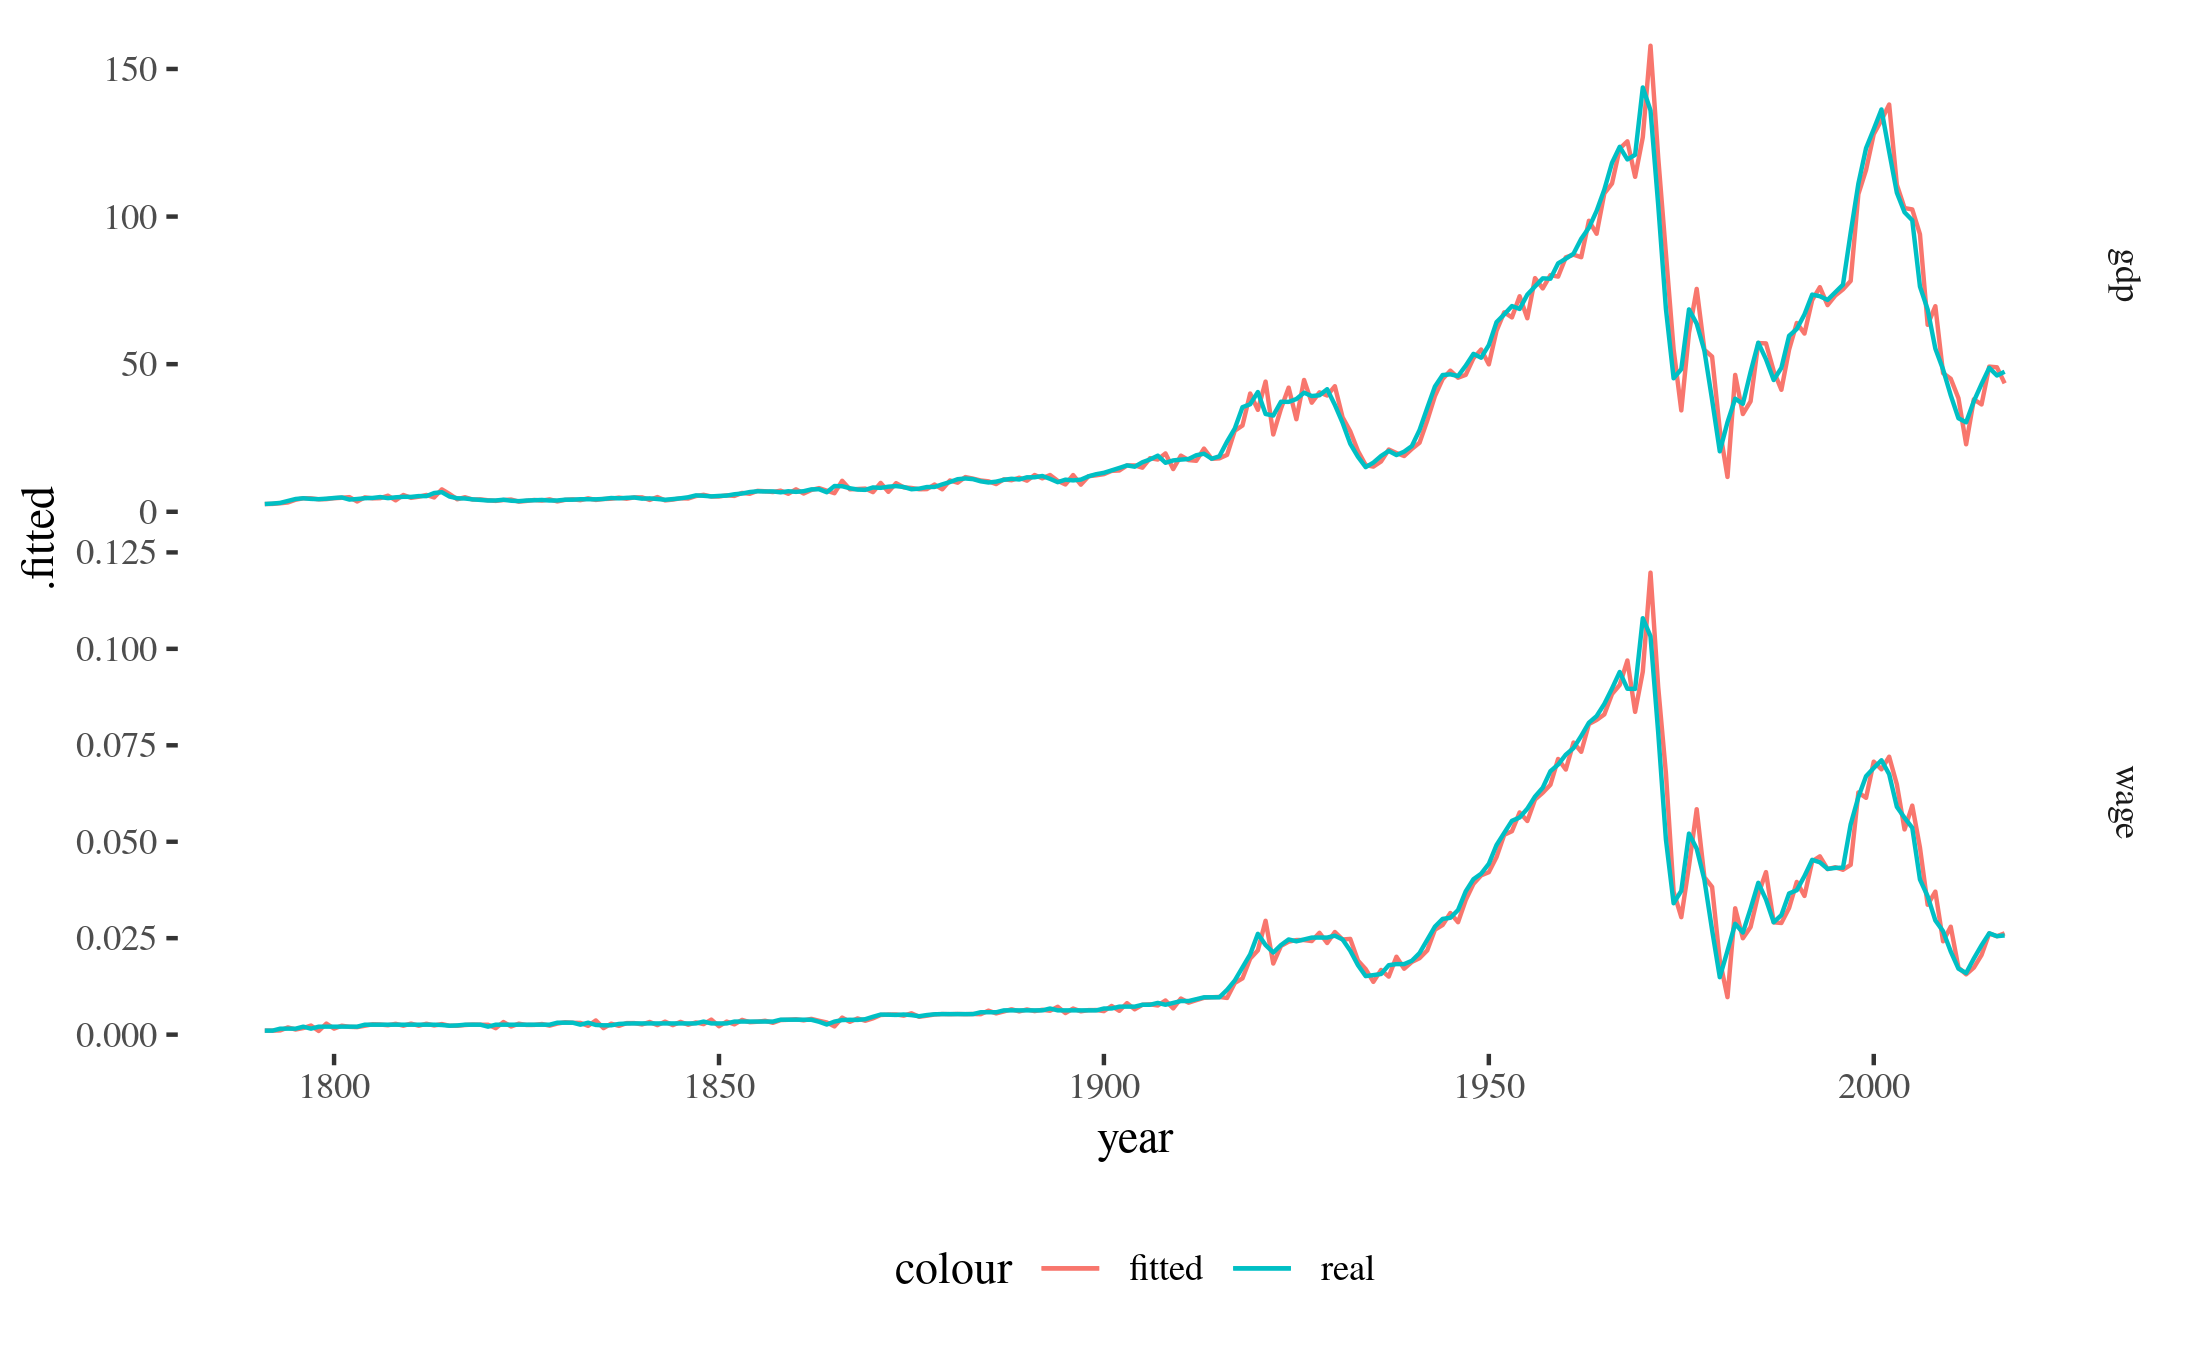
\includegraphics[width=0.8\linewidth]{arima_tot.png}
	\label{fig:arima_tot}}
	\subfigure[ARIMA por grupos]{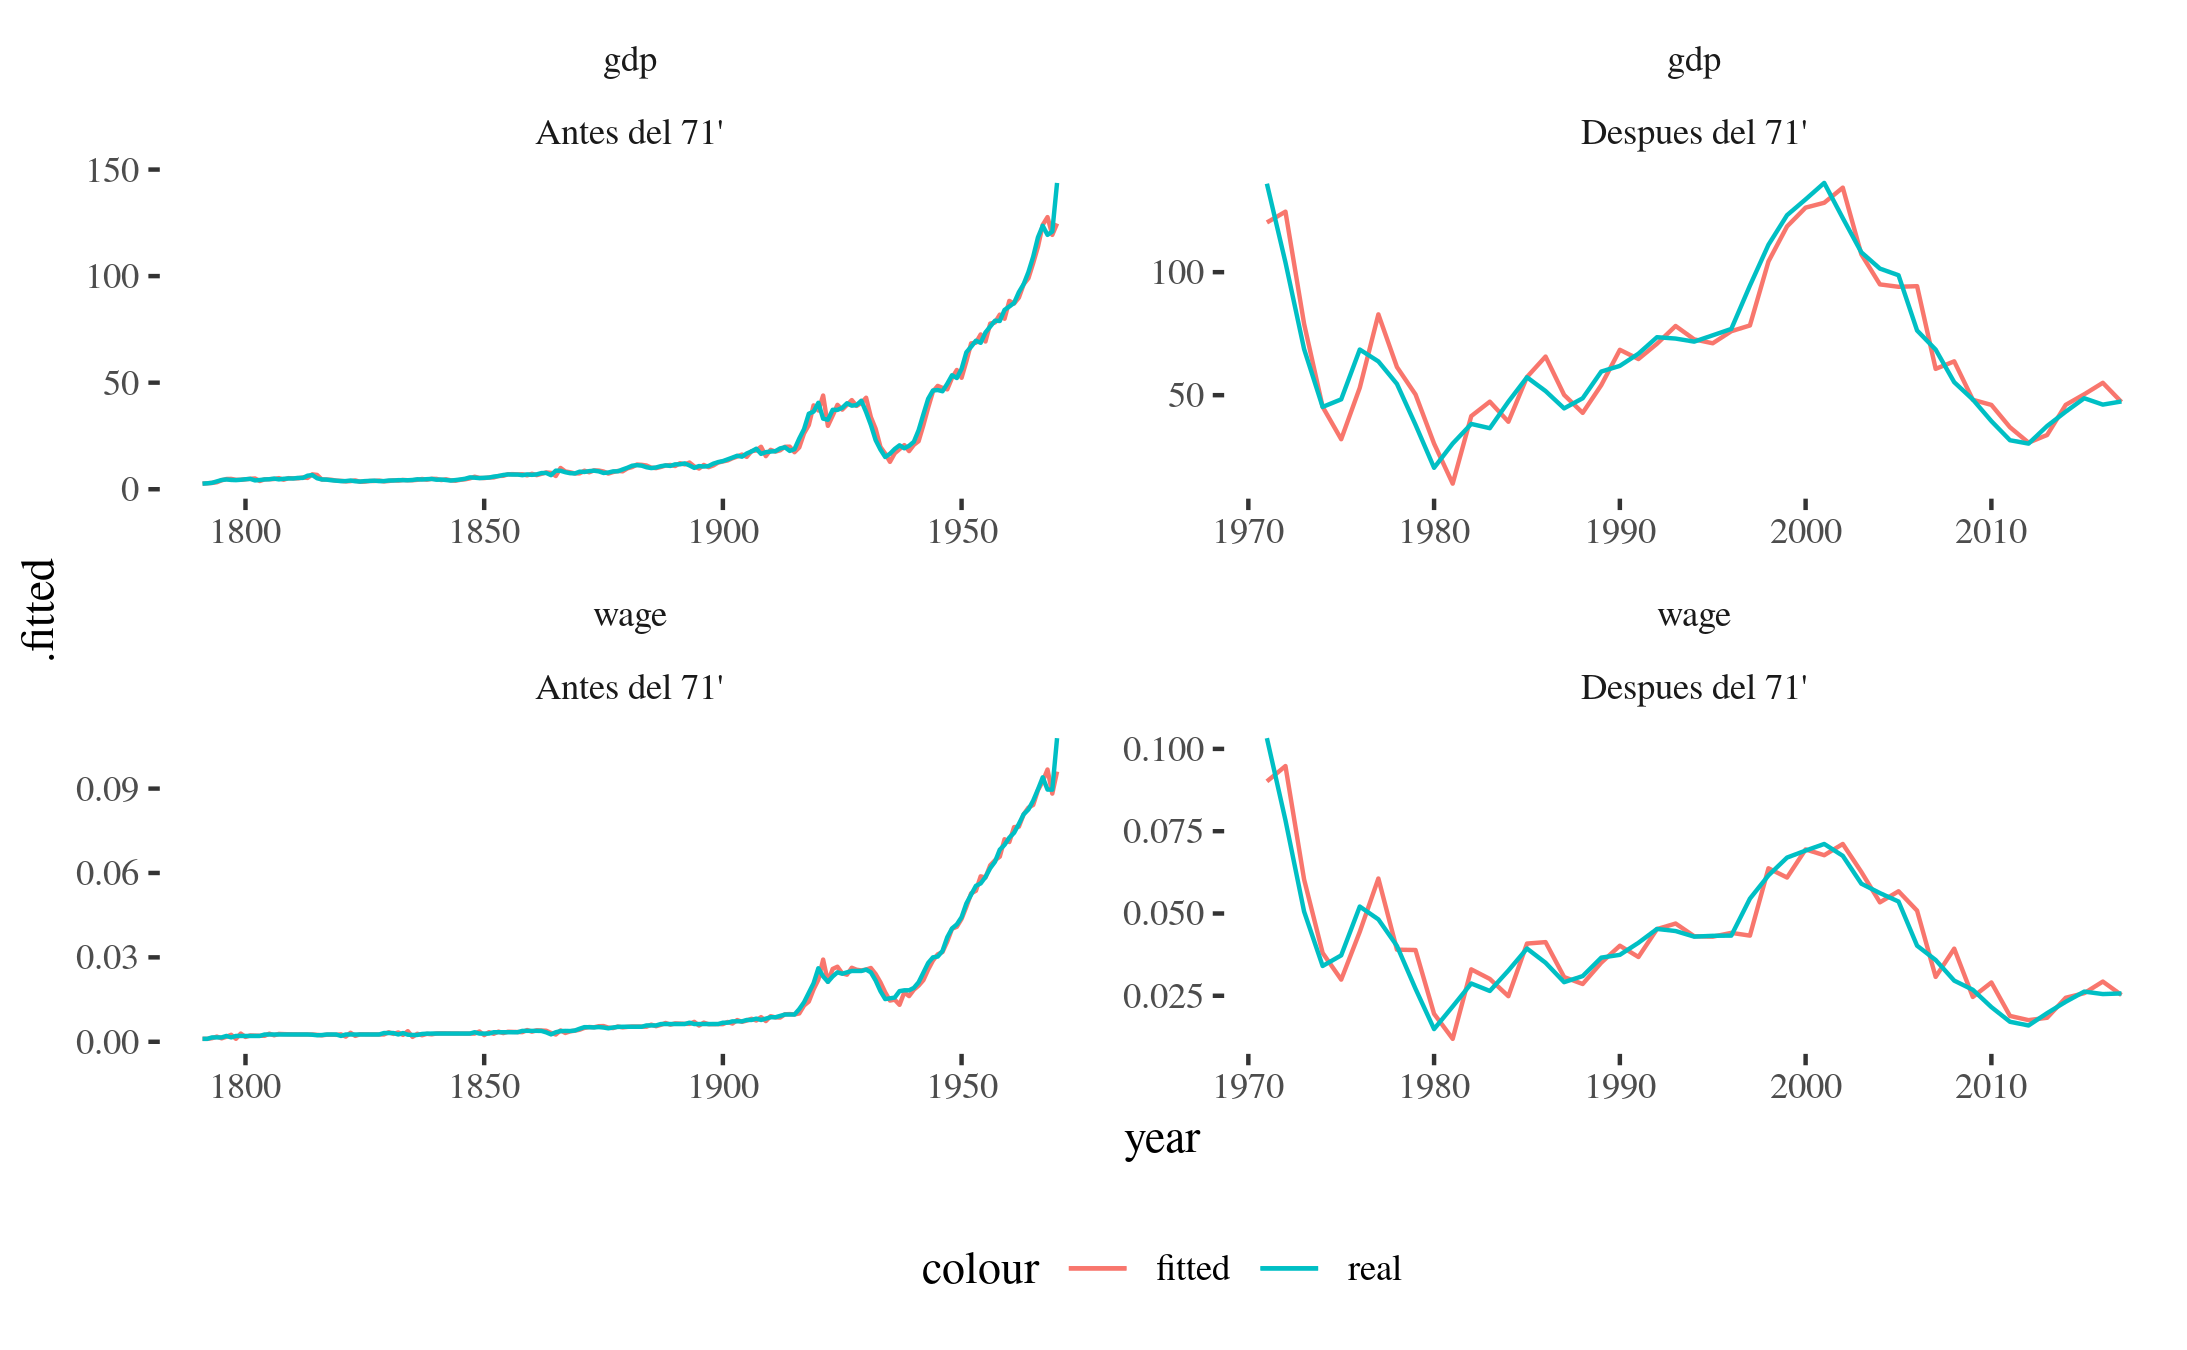
\includegraphics[width=0.8\linewidth]{arima_groups.png}
	\label{fig:arima_grp}}
	\caption{Predicción ARIMA} \label{fig:arima}
\end{figure}

Lo observado en \ref{fig:arima_grp} son los siguientes cuatro modelos: 

\begin{table}[ht]
	\centering
	\begin{tabular}{rlllrr}
		\hline
		& tipo & group & model.desc & sigma & RMSE \\ 
		\hline
		1 & wage & Antes del 71' & ARIMA(2,2,1) & 0.00 & 0.00 \\ 
		2 & wage & Despues del 71' & ARIMA(1,0,2) with non-zero mean & 0.01 & 0.01 \\ 
		3 & gdp & Antes del 71' & ARIMA(0,2,2) & 2.48 & 2.45 \\ 
		4 & gdp & Despues del 71' & ARIMA(2,0,0) with non-zero mean & 9.59 & 9.27 \\ 
		\hline
	\end{tabular}
\end{table}

Se observa tanto un mayor desvío como un mayor error cuadrático medio para ambas series después de 1971. A su vez, las series antes del 71' son integradas de orden dos, producto de lo mencionado arriba de que hasta este punto se toma la fuerte fase ascendente del ciclo en la posguerra, en y lo convierte en una serie divergente. Al contrario, los ARIMA óptimos para las series posteriores a 1971 no requieren ser integrados, sino simplemente tener un término de nivel (\textit{non-zero mean}). A su vez, el modelo también pareciera ser más volátil que las observaciones en este período. Como conclusión, estas herramientas tradicionales de la econometría no bastan para dar cuenta del fenómeno cíclico. 

\section{Wavelets}

Por lo anterior, se decidió explorar nuevas herramientas del análisis de series de tiempo para poder caracterizar el ciclo económico. En particular, los espectogramas producidos mediante \textit{wavelets} parecen ser una herramienta propicia para encontrar ciclos bien definidos a lo largo del período analizado. Para ello, comenzamos definiendo un modelo teórico de una economía cíclica, con los diferentes componentes vistos de por separado y en su composición, para observar las características del espectograma en este modelo,  y luego compararlo con los datos reales. 
En la figura \ref{fig:serie_teorica} se observan 100 valores de los distintos componentes con los que construiremos la serie:

\begin{itemize}
	\item \textbf{impulso}: Una serie con un valor constante de 50, que en período en particular tomar el valor 100.
	\item \textbf{Tendencia}
	\item \textbf{ciclo corto}: Un ciclo de amplitud y extensión pequeña
	\item \textbf{ciclo medio}: Un ciclo de amplitud y extensión media
	\item \textbf{ciclo largo}: Un ciclo de amplitud y extensión grande
	\item \textbf{ruido}: Ruido generado a partir de una distribución normal, poco significativo respecto a la amplitud de los ciclos y la pendiente de la tendencia.
\end{itemize}

\begin{figure}[H]
	\centering
	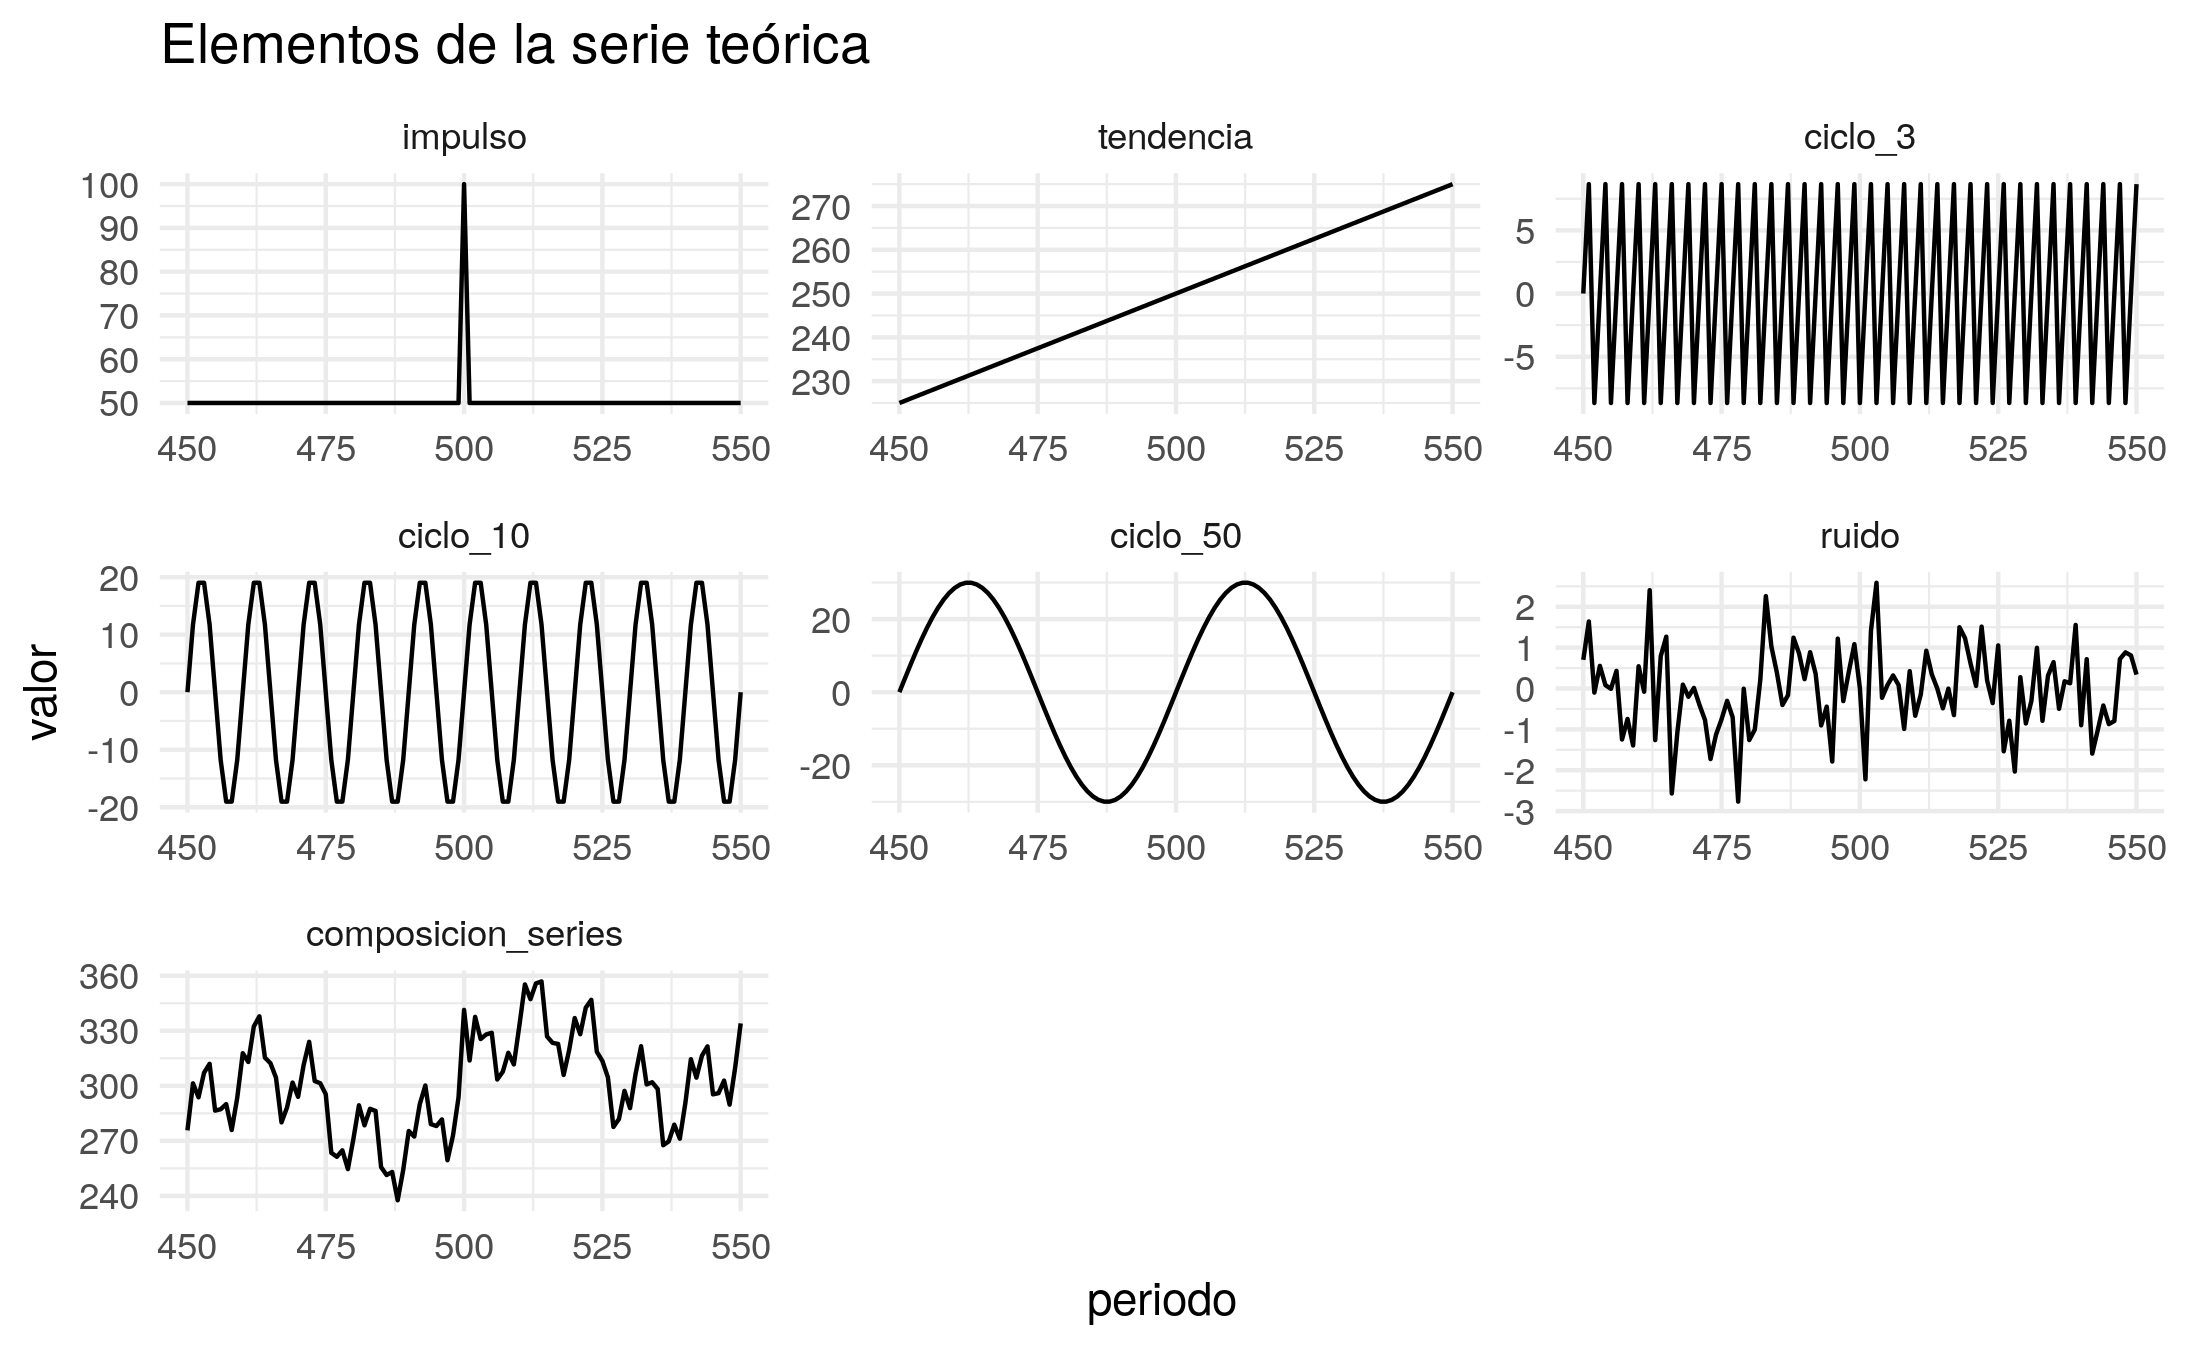
\includegraphics[width=\linewidth]{serie_teorica.PNG}
	\caption{Serie Teórica} \label{fig:serie_teorica}
\end{figure}

En la figura \ref{fig:espect_teo} se observa el espectograma de cada uno de los elementos mencionados. Dicho gráfico muestra en el eje vertical el período, la inversa de la frecuencia de onda, que corresponde a la distancia entre los valles o picos de un ciclo. La escala cromática (de los azules para los valores más bajos a los rojos en los valores más altos) representa la amplitud del ciclo. el eje horizontal representa el tiempo calendario. Es decir, para cada tiempo calendario podemos observar la amplitud del ciclo en cada una de las posibles frecuencias de onda. El impulso se presenta como un ciclo de amplitud grande en todas las frecuencias, en el momento correspondiente. La tendencia, por su parte, se presenta básicamente como ruido, dado que es estrictamente un comportamiento no cíclico. Sin embargo, presenta la particularidad de presentar valores de amplitud mayores hacia el final del período para frecuencias basjas, y valores de amplitud particularmente bajos en las frecuencias altas de los primeros momentos.
Los tres ciclos definidos marcan claramente una línea horizontal en el correspondiente período, que luego se diluye hacia las demás frecuencias. Finalmente, el normal presenta un comportamiento muy particular, mostrando mayores amplitudes, de forma irregular, en las frecuencias altas, y homogeneizándose hacia valor de amplitud baja en las frecuencias más bajas. Esto se debe a que el ruido normal se puede parecer a un ciclo de períodos muy cortos debido a una sucesión de subas y bajas, pero dado que es aleatorio es cada vez más improbable que se asemeje a ciclos de períodos mayores, dado que ello implicaría una mayor cantidad de sucesiones de subas y bajas. 
Por último, en la composición se series se observa como los ciclos de mayor amplitud y frecuencia se expresan en la escala cromática de forma más nítida que los ciclos de menor amplitud y frecuencia. Es importante resaltar que la concordancia entre amplitud y frecuencia es producto de la forma en que construimos las series, dado que esperamos que los ciclos económicos más largos se correspondan también con movimientos de mayor amplitud.

Vale mencionar que la elección para el modelo teórico de estos tres niveles y amplitudes cíclicas no es arbitraria, sino que se corresponde con lo considerado por la literatura: \cite{kondratieff1979long} estudia las series largas, de unos 50 años, mientras que \cite{kuznets1930secular} propone movimientos seculares de entre 15 y 25 años. Finalmente el Real business cycle \citep{kydland1982time} considera un ciclo corto. Por ello, decidimos modelar ciclos de 50, 10 y 3 años. 

\begin{figure}[H]
	\centering
	\subfigure[impulso]{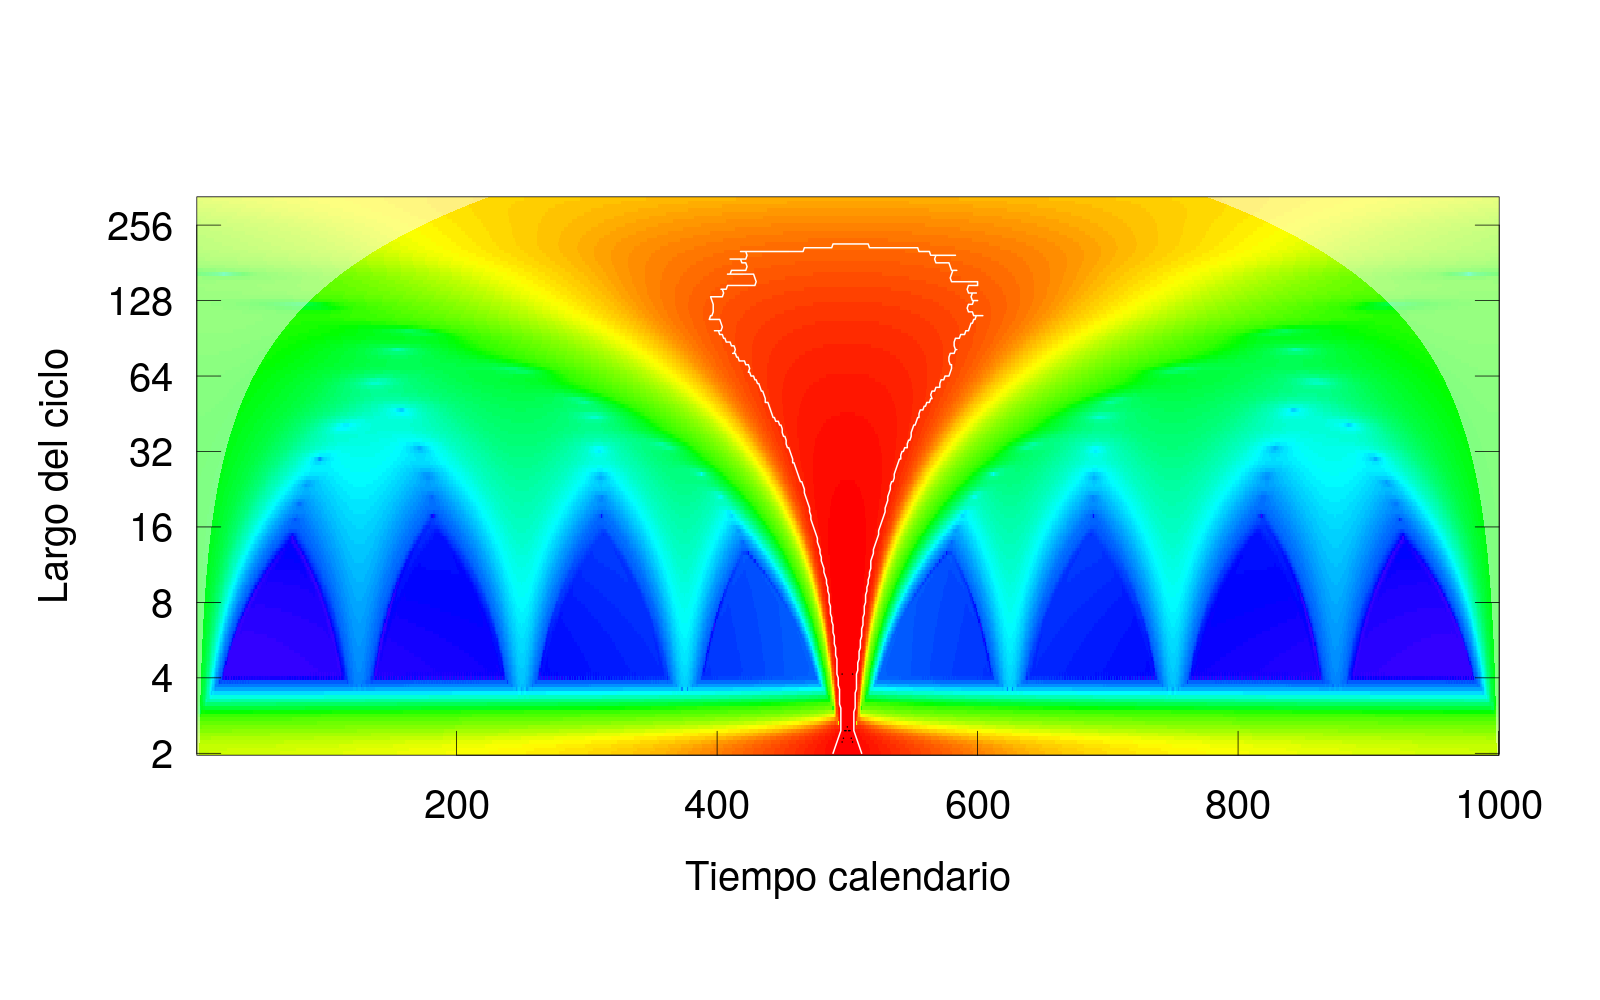
\includegraphics[width=0.49\linewidth]{espectograma_teorico_impulso.png}}
	\subfigure[tendencia]{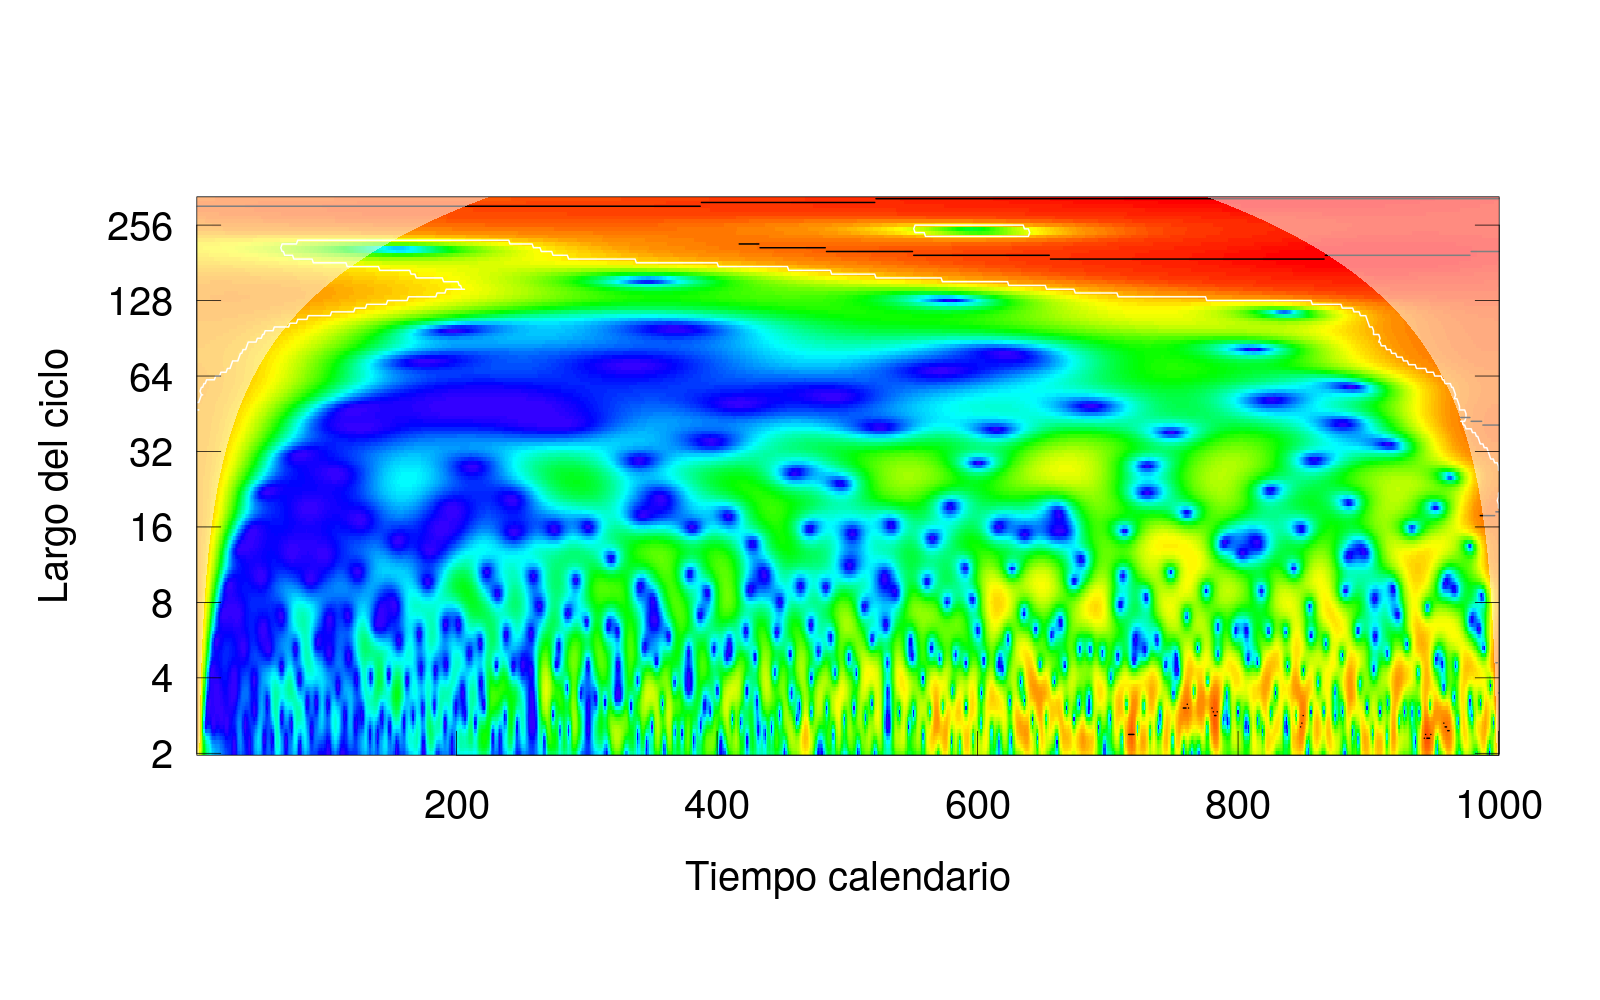
\includegraphics[width=0.49\linewidth]{espectograma_teorico_tendencia.png}}
	\subfigure[ciclo de 3 años]{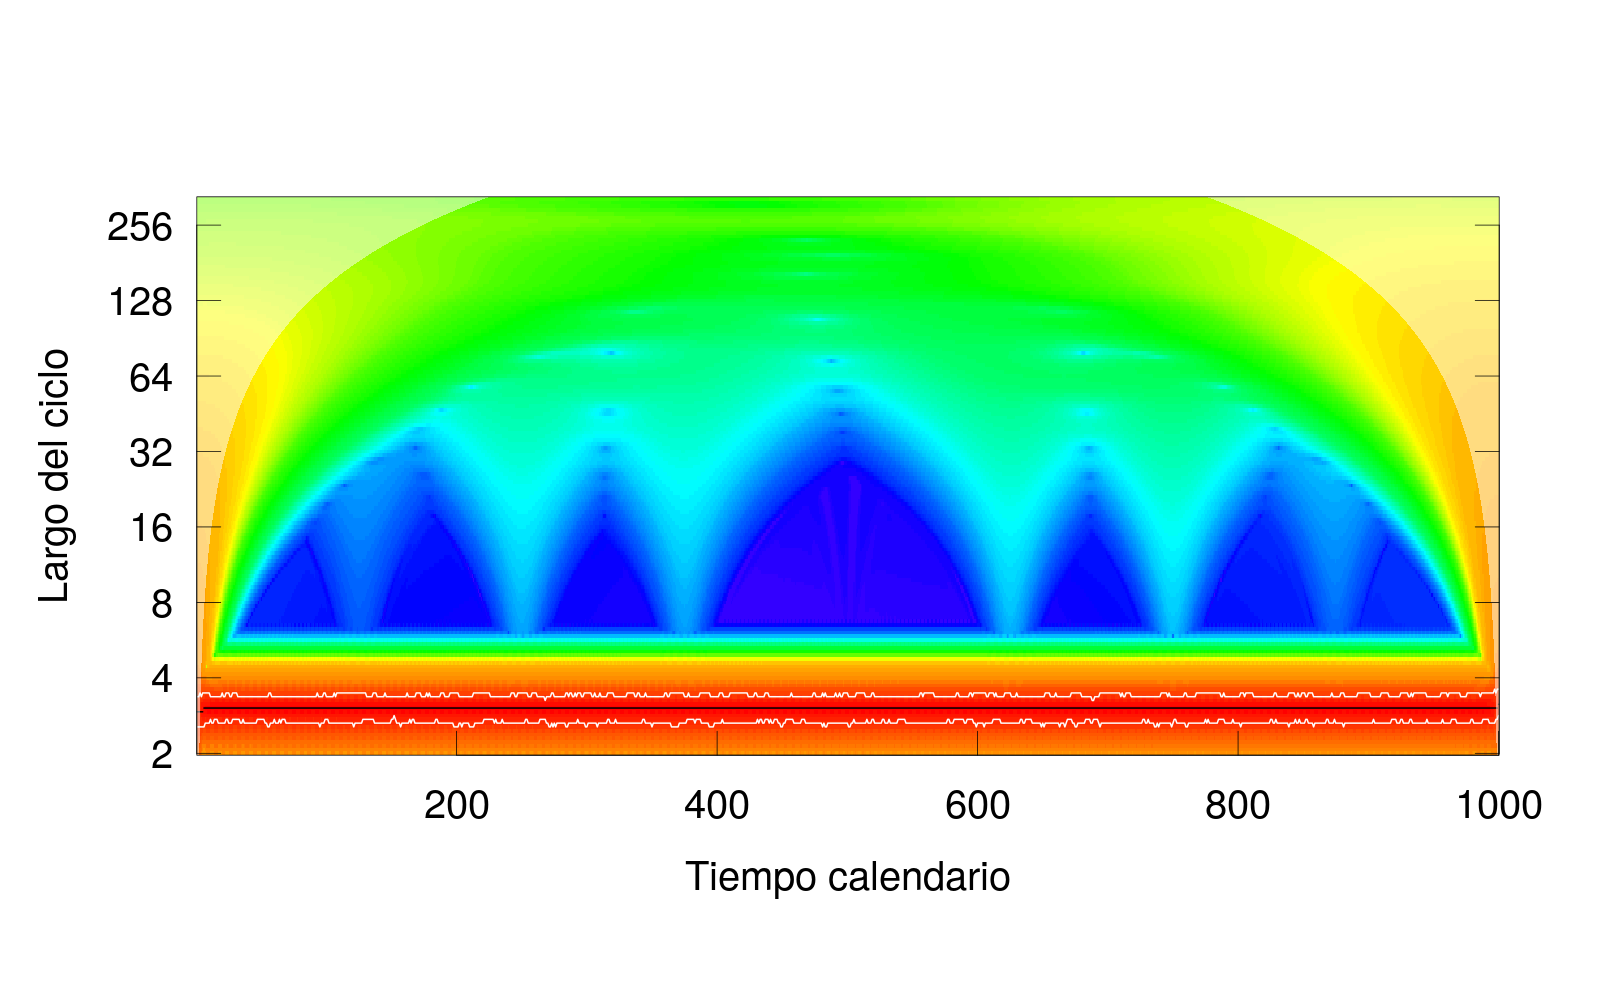
\includegraphics[width=0.49\linewidth]{espectograma_teorico_ciclo_3.png}}
	\subfigure[ciclo de 10 años]{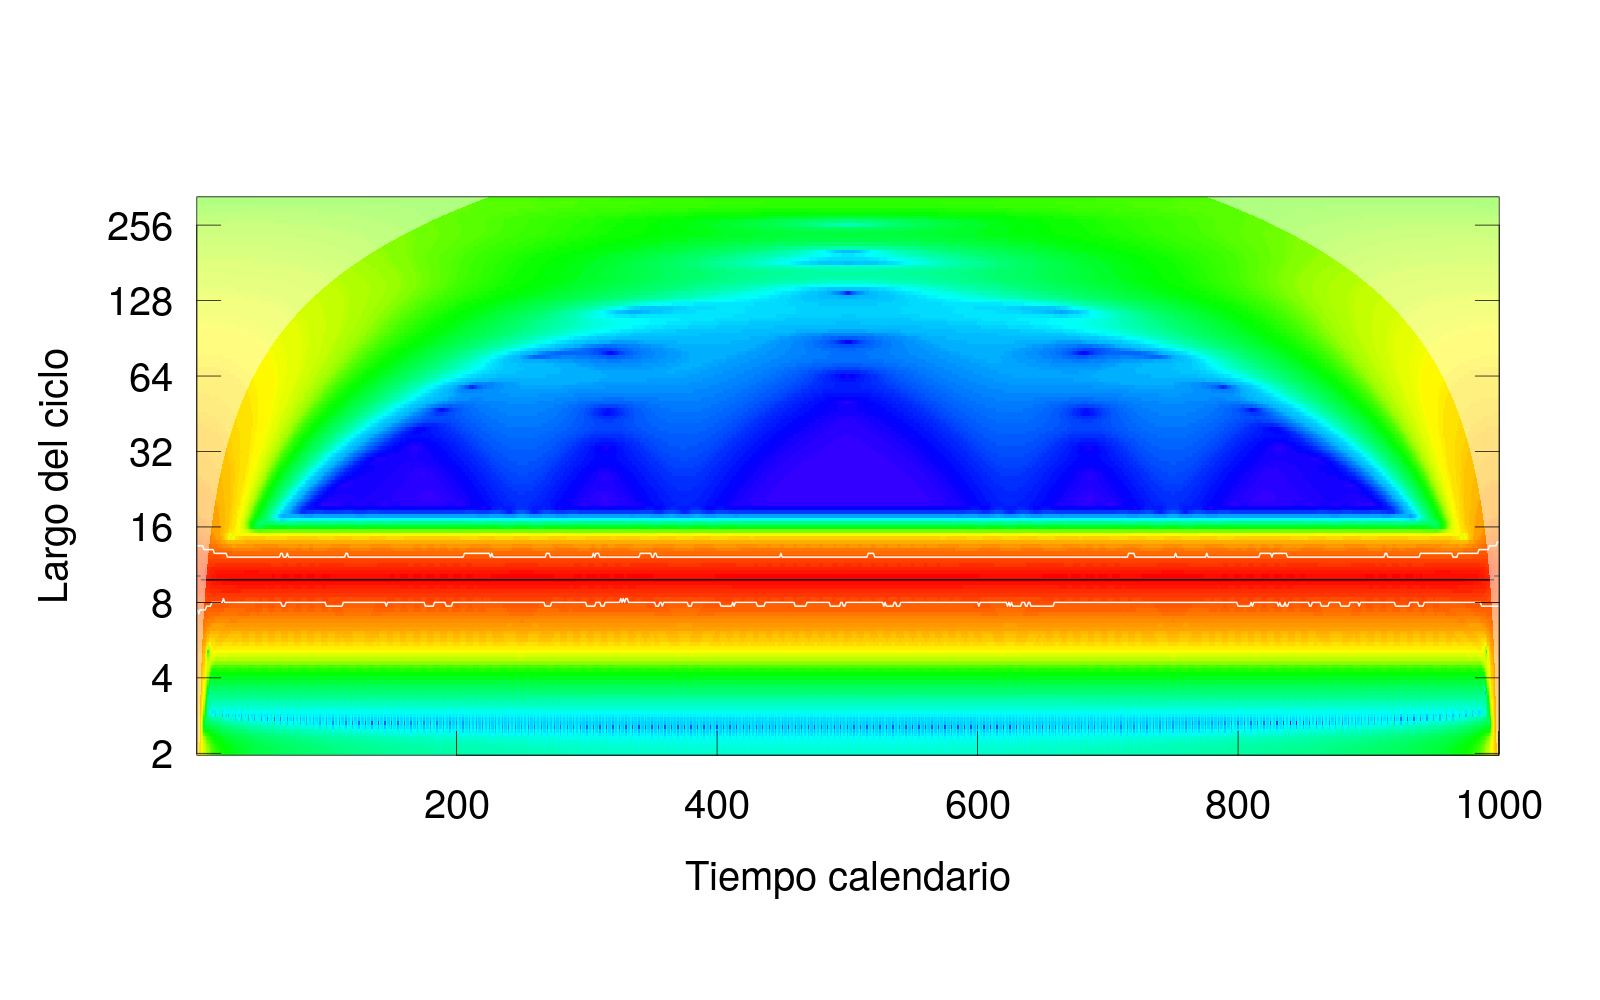
\includegraphics[width=0.49\linewidth]{espectograma_teorico_ciclo_10.png}}
	\subfigure[ciclo de 50 años]{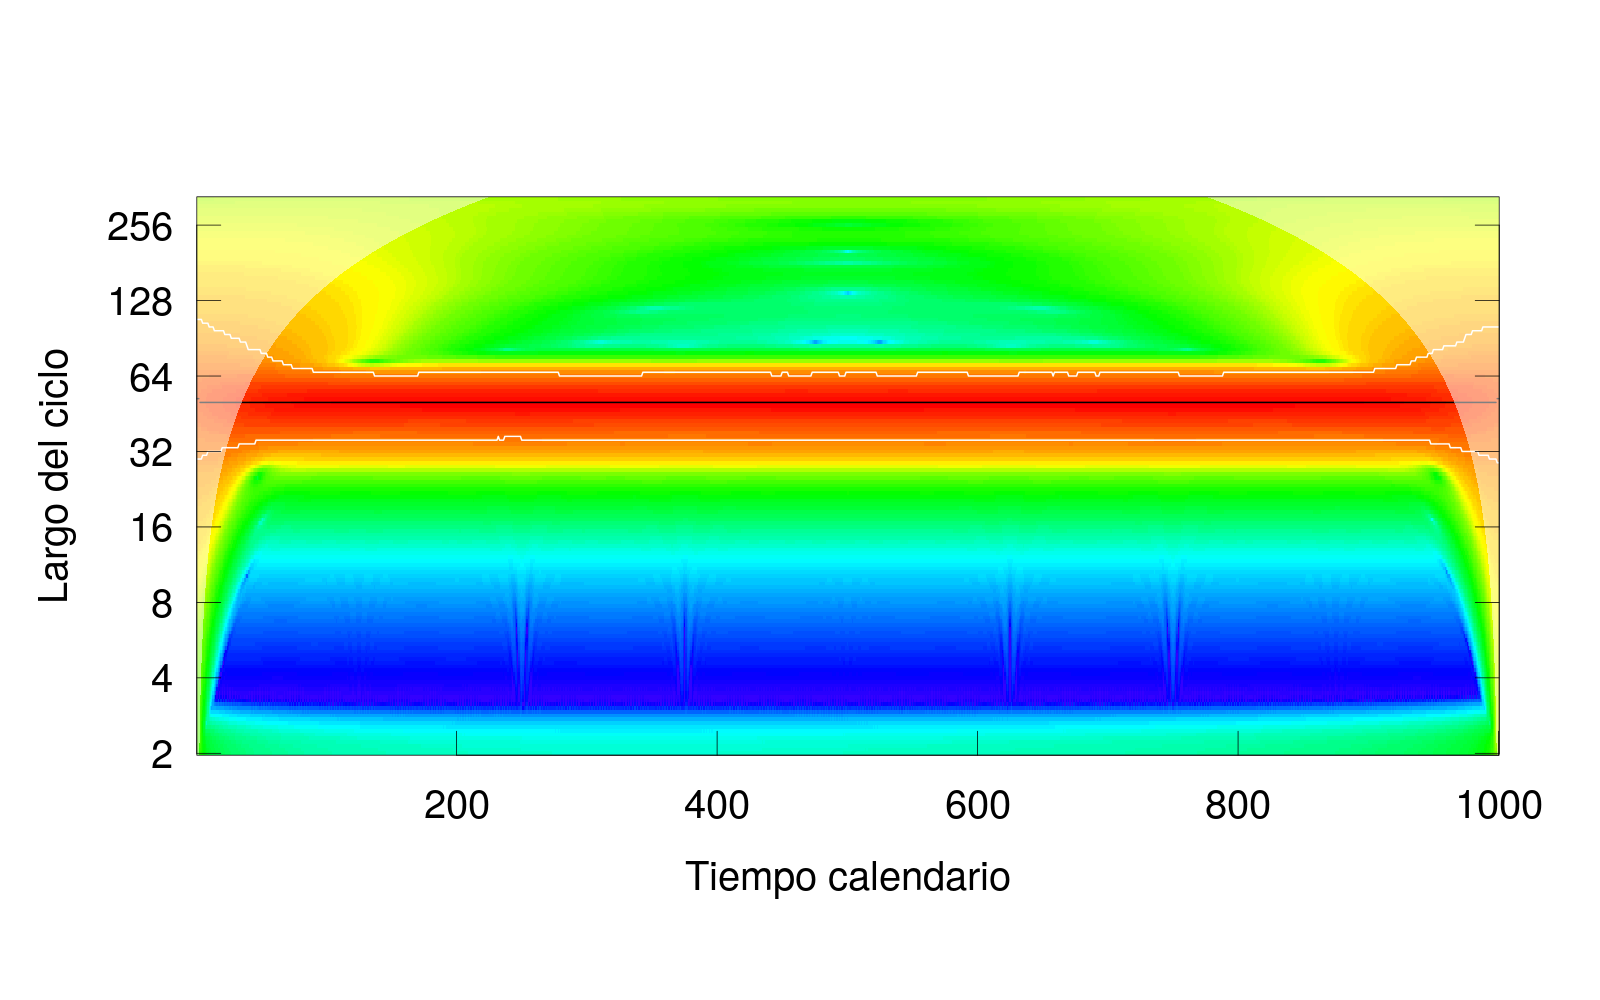
\includegraphics[width=0.49\linewidth]{espectograma_teorico_ciclo_50.png}}
	\subfigure[ruido normal]{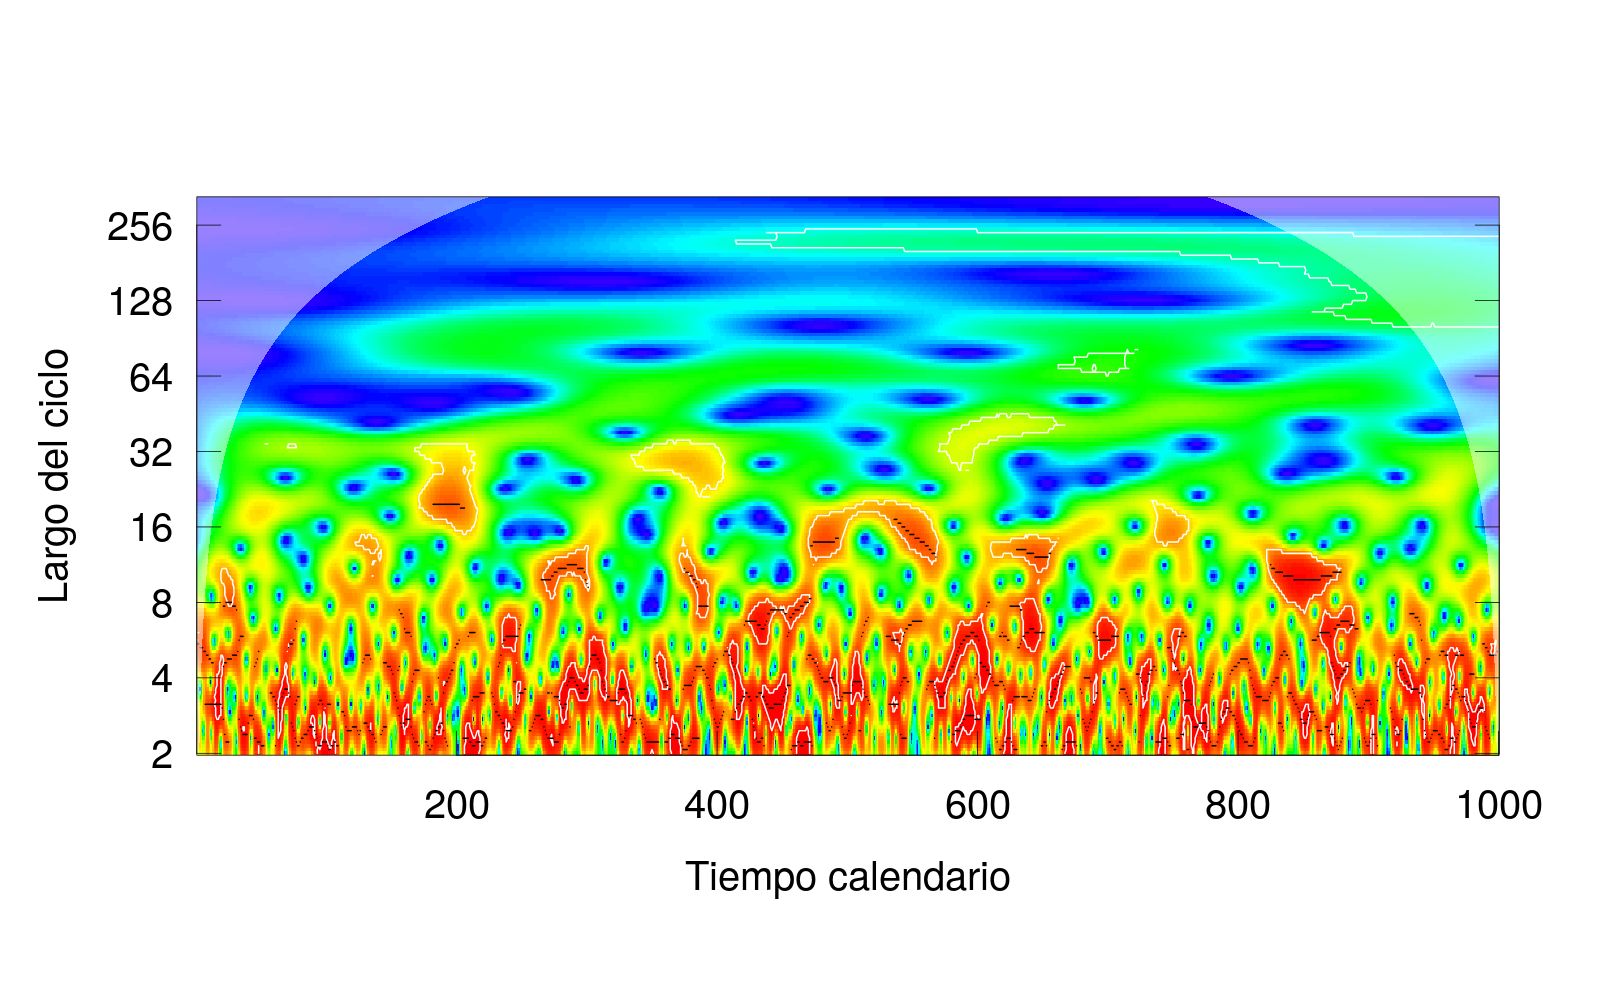
\includegraphics[width=0.49\linewidth]{espectograma_teorico_ruido.png}}
	\subfigure[composición de series]{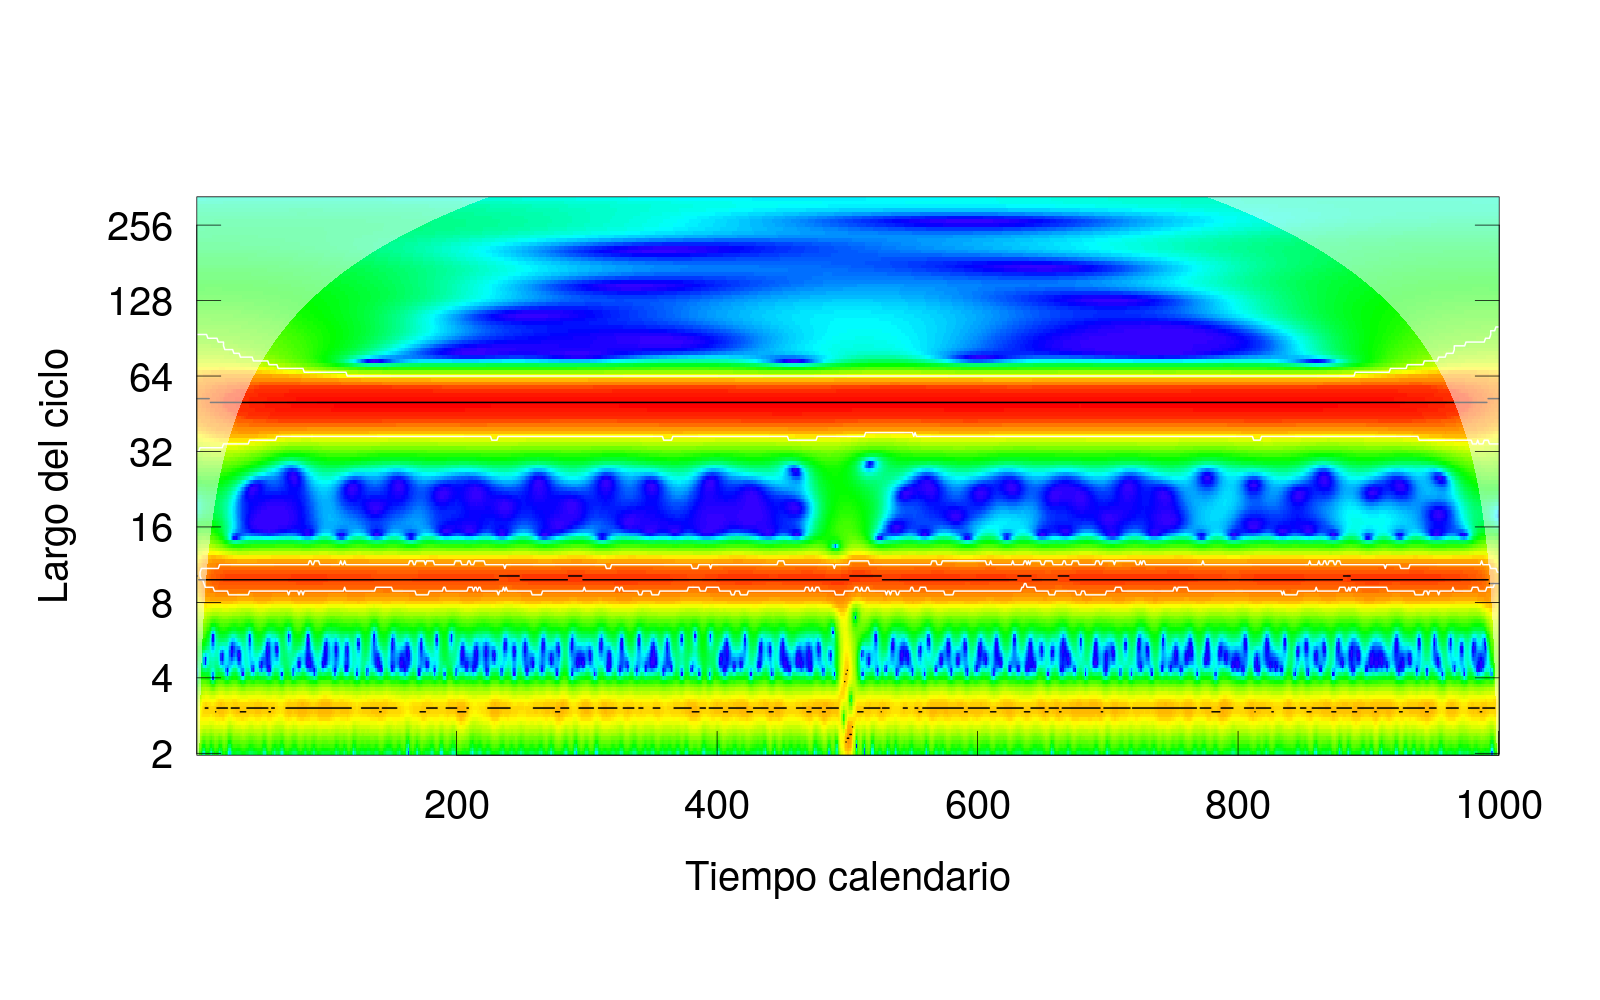
\includegraphics[width=0.75\linewidth]{espectograma_teorico_composicion_series.png}}
	\caption{Espectogramas Teóricos} \label{fig:espect_teo}
\end{figure}

Con lo analizado de la figura \ref{fig:espect_teo} podemos observar los resultados de las series originales. En la figura \ref{fig:espect_PBI_a} se puede observar el espectograma correspondiente al PBI de estados unidos expresado en oro. Allí se marca claramente la diferencia en la serie antes y después del 1900, y en particular también se marca el quiebre estudiado de los años 70'. No obstante lo cual, para ese período se observan 3 frecuencias donde se registra un comportamiento cíclico, en los períodos aproximados de 8 y 50 años, y un ciclo diferenciado de este último, de aproximadamente 30 años. Dada la heterocedasticidad de las series, en \ref{fig:espect_PBI_b} se propone el espectograma de la misma serie tomada en logaritmo de base 10. De esta forma lo que se observa es que el ciclo de 50 años se extiende más allá en el tiempo, hasta mediados del S XIX. Por su parte, aparece brevemente un ciclo más corto, de aproximadamente tres años, en la década del 70.

\begin{figure}[H]
	\centering
	\subfigure[PBI]{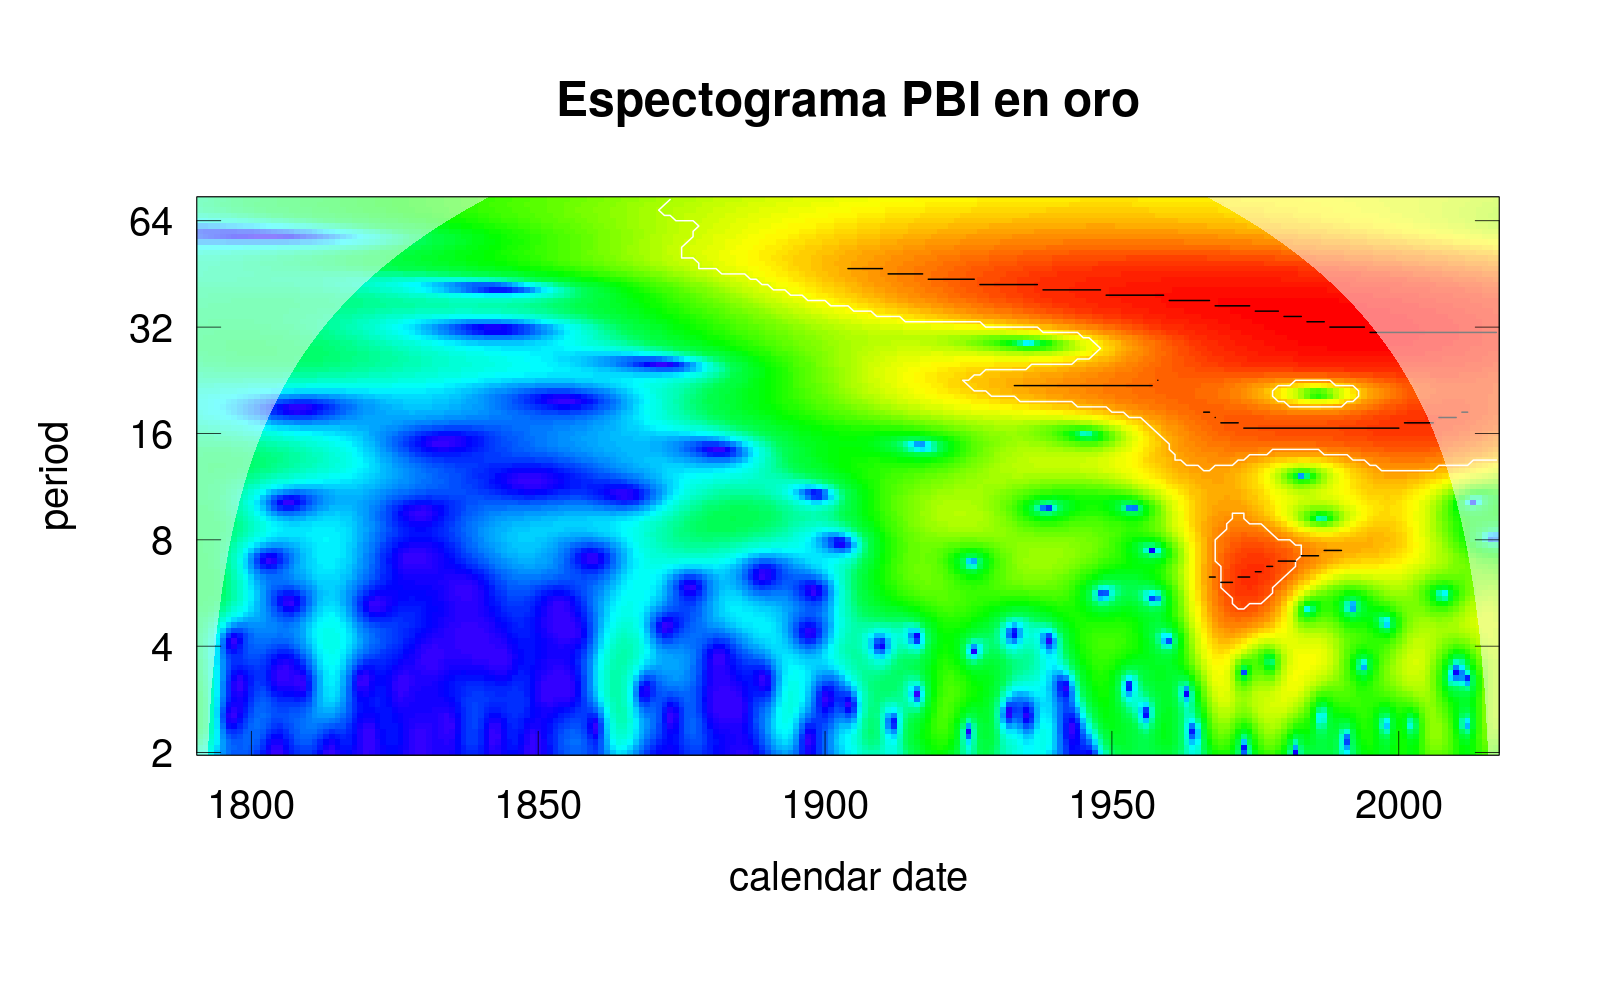
\includegraphics[width=0.75\linewidth]{espectograma_gdp.png}
	\label{fig:espect_PBI_a}}
	\subfigure[$log(PBI)$]{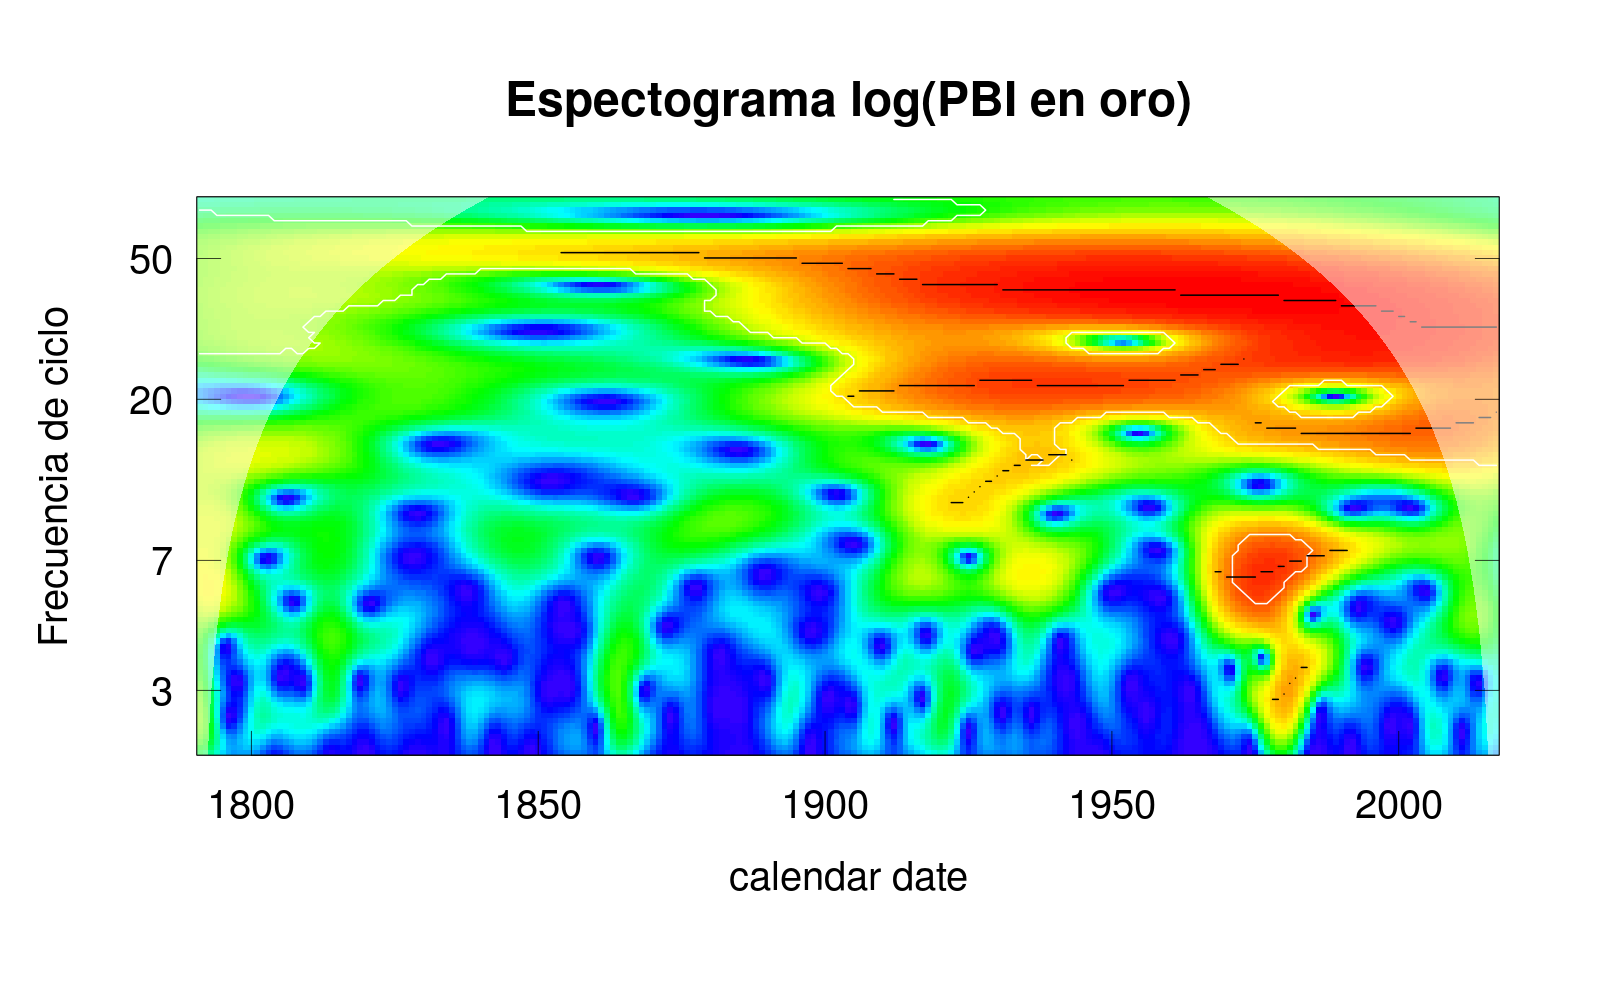
\includegraphics[width=0.75\linewidth]{espectograma_log_gdp.png}
	\label{fig:espect_PBI_b}}
	\caption{Espectograma PBI en oro} \label{fig:espect_PBI}
\end{figure}

las figuras \ref{fig:espect_wg} muestran los espectogramas de la serie del salario expresado en oro \ref{fig:espect_wg_a} y el mismo tomado en logaritmo en \ref{fig:espect_wg_b}. Para esta serie nuevamente se observa un ciclo largo bien definido en torno a los 50 años, especialmente si se observa la serie tomada en base logarítmica. Este ciclo largo parece oscilar entre las frecuencias de $1/32$ y $1/64$, cayendo en el tiempo. Pos su parte, se delimita un segundo ciclo, en torno a los 16 años de extensión, y finalmente un ciclo corto de entre 6 y 8 años.  Al tomar la escala logarítmica, también aparece un ciclo de mayor frecuencia, de unos 3 años de duración. 

\begin{figure}[H]
	\centering
	\subfigure[Salario]{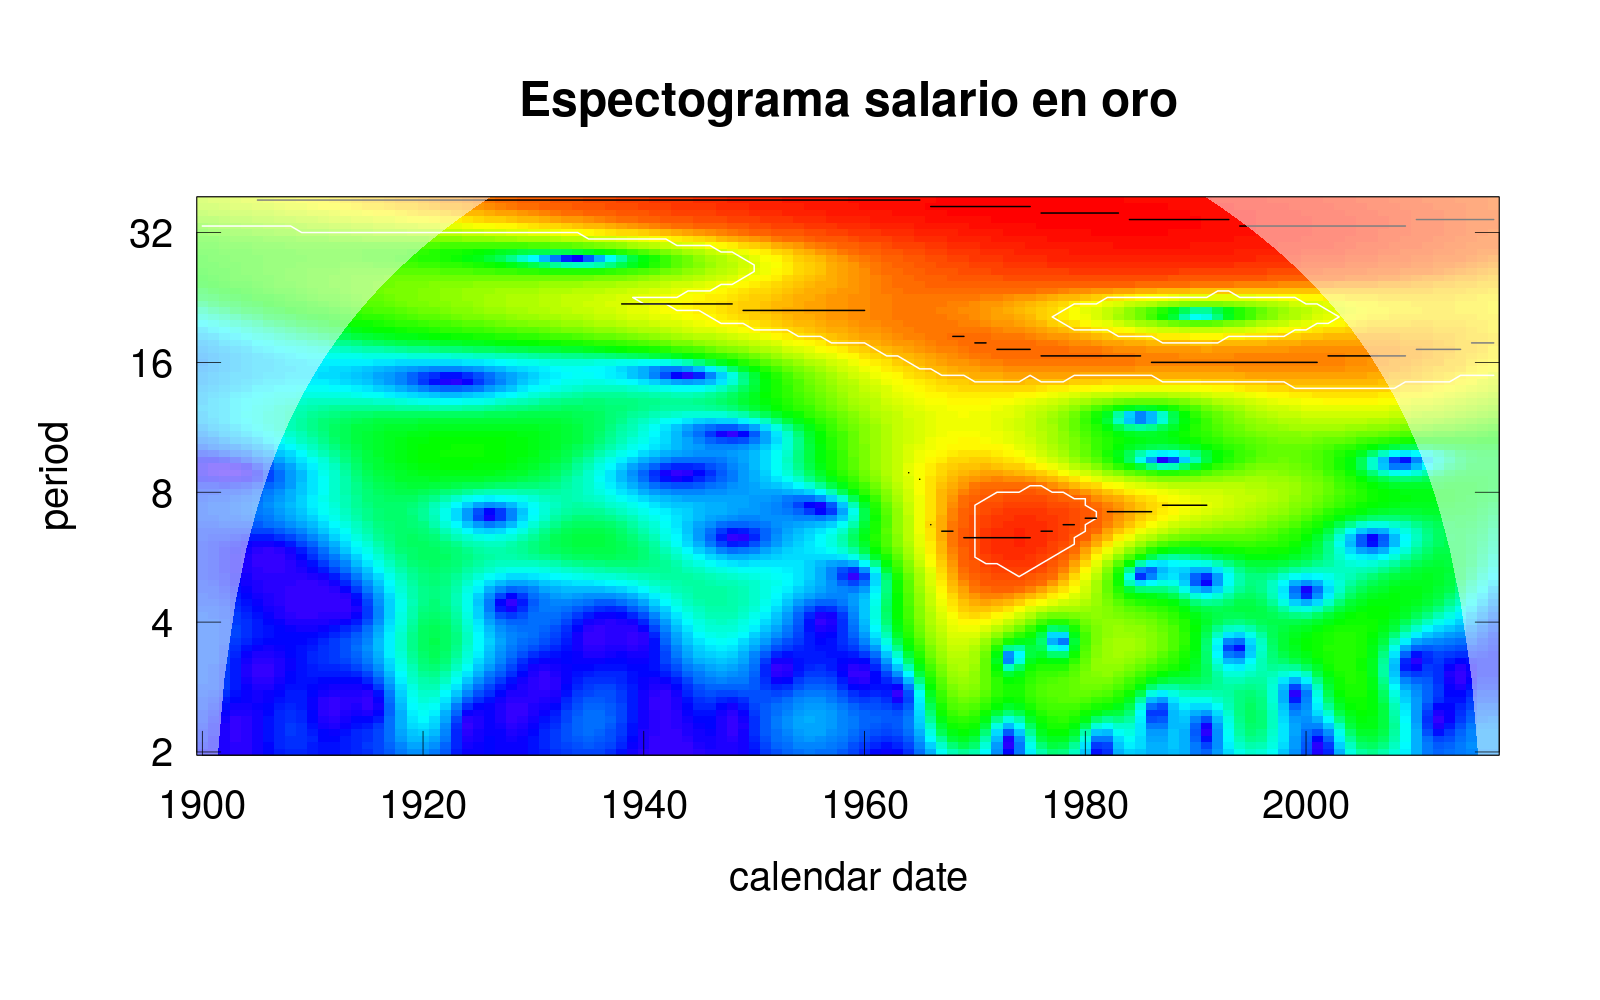
\includegraphics[width=0.75\linewidth]{espectograma_wg.png}
	\label{fig:espect_wg_a}}
	\subfigure[$log(Salario)$]{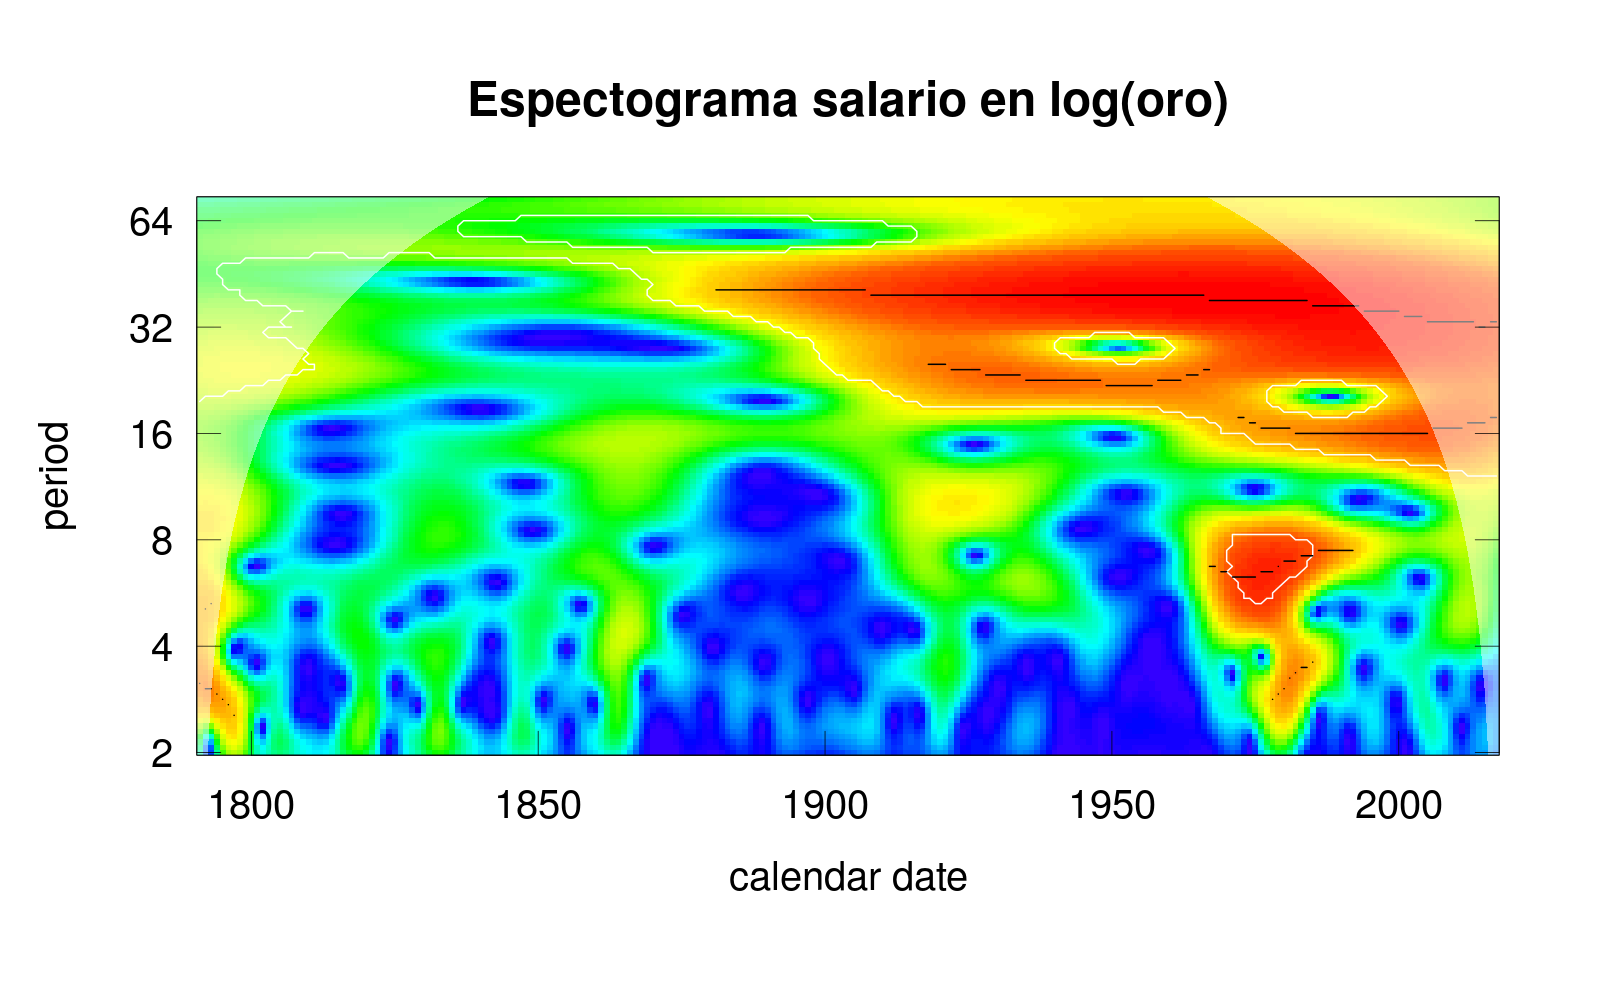
\includegraphics[width=0.75\linewidth]{espectograma_log_wg.png}
	\label{fig:espect_wg_b}}
	\caption{Espectograma Salario en oro} \label{fig:espect_wg}
\end{figure}



\section{Conclusiones}

\todo{falta}

Es interesante remarcar el siguiente punto: el objetivo del presente trabajo es buscar evidencia empírica respecto de la frecuencia y amplitud del comportamiento cíclico de la economía. Se toma las series de salario y PBI por ser buenos aproximadores de movimiento económico general, pero no son los únicos. A su vez, como las estadísticas tienen una base nacional, el PBI siempre es de un país en particular, así como las estadísticas del salario, debimos decidir tomar un país particular, como expresión de la economía mundial. En este sentido, al ser Estados Unidos la unidad nacional de la economía mundial de mayor envergadura, optamos por este país como representante de la economía mundial. No obstante, si bien la economía estadounidense es un buen reflejo de los movimientos de la economía mundial durante el siglo XX, lo mismo no se sostiene para el siglo XIX, dado que no se había constituido aún como la primera potencia de la economía mundial. En este sentido, es natural que no se expresen las determinaciones generales de la economía, como el ciclo, para dicho siglo, y observemos evidencia sólo a partir del 1900.


\bibliography{bibliography.bib}


\end{document}